\chapter{Neural Network Performance And Benchmarking}
\label{ch:performance_benchmarks}

%%%%%%%%%%%%%%%%%%%%%%%%%%%%%%%%%%%%%%%%%%%%%%%%%
\section{Experimental Setup And Evaluation Protocol}
\label{sec:benchmark_protocol}
This chapter reports the final empirical comparison of the neural models developed in the thesis. The results are organized around two methodological branches. The first branch is supervised and works with implied-volatility labels: it includes the ANN baseline and the ANN Sobolev variant, together with the CaNN calibration workflow that uses the trained ANN surrogate as a fast evaluator. The second branch is physics-informed and works directly in price space: it includes the PINN baseline, the PINN Sobolev variant, and the PINN Sobolev variant including an analytical control variate (ACV) correction.

Unless explicitly stated, all reported metrics are computed on fixed evaluation sets with identical feature conventions, consistent preprocessing, and the same numerical references used in previous chapters.

\subsection{Primary Error Metrics}
\label{sec:benchmark_error_metrics}

To keep the empirical comparison coherent, the chapter uses three primary error metrics throughout: MSE, RMSE, and MAPE. Let \(z_i^{\mathrm{ref}}\) be the reference value and \(\hat z_i\) the model value at evaluation point \(i\), for \(i=1,\ldots,n\). The metrics are
\begin{equation}
    \begin{aligned}
    \mathrm{MSE}
        &=\frac{1}{n}\sum_{i=1}^{n}\left(\hat z_i-z_i^{\mathrm{ref}}\right)^2,\\
    \mathrm{RMSE}
        &=\sqrt{\mathrm{MSE}},\\
    \mathrm{MAPE}
        &=100\,\frac{1}{n}\sum_{i=1}^{n}
        \frac{\left|\hat z_i-z_i^{\mathrm{ref}}\right|}
        {\max\left(\left|z_i^{\mathrm{ref}}\right|,\varepsilon_{\mathrm{MAPE}}\right)}.
    \end{aligned}
\end{equation}
MSE is aligned with the training objective used in the supervised components, RMSE restores the error to the natural output units, and MAPE provides a scale-relative percentage reading. The denominator floor \(\varepsilon_{\mathrm{MAPE}}\) avoids unstable ratios near zero. Tail quantiles and maximum errors are used only as auxiliary diagnostics when discussing distributional behavior, not as headline metrics.

The minimal pre-benchmark validation protocol combines three checks: convergence with respect to \((N,L)\) in the COS expansion, put-call parity residual control across strikes, and Black--Scholes consistency in near-constant-variance regimes.

These checks are used as a guardrail before comparing models, so that downstream differences can be attributed to model behavior rather than to numerical artifacts. For consistency across Sections~\ref{sec:ann_pricer_performance}--\ref{sec:pinn_greeks_performance}, each block is analyzed with the same reading logic: global summary metrics, localized error diagnostics over relevant domains, and runtime indicators.

The protocol is fixed as follows. Randomness is controlled with a common seed (\(42\)) in data generation and training configurations; in calibration, the Differential Evolution seed follows the same base value unless explicitly overridden. The Heston domain is shared across experiments, with \(\rho\in[-0.9,0]\), \(\kappa\in[0,3]\), \(\gamma\in[0.01,0.8]\), \(\bar v\in[0.01,0.5]\), \(v_0\in[0.05,0.5]\), and contract coordinates \(m\in[0.6,1.4]\), \(\tau\in[0.05,3.0]\) for ANN/CaNN benchmarks. Reference numerics are also fixed: COS pricing with \(N=1500\), \(L=50\), and fallback \(L=80\) when required by stability checks, plus Brent IV inversion with \(\mathrm{tol}=10^{-8}\) and bounded search interval.

Reported metrics are always computed on fixed evaluation sets. For the supervised ANN branch, the split policy is fixed to \(0.8/0.1/0.1\) (train/validation/test). For the PINN branch, the collocation data use a train/validation split rather than supervised labels; the final configurations use \(0.8/0.2\), and pricing or Greek metrics are then reported on fixed benchmark grids. Values are reported in decimal units (IV for ANN/CaNN, price for PINN). These units are not used to build a direct ANN-versus-PINN ranking: ANN results are read in implied-volatility space, with price or Greek diagnostics reported as derived quantities, whereas PINN results are read first in price space and then through separate Greek diagnostics.

Methodological details are kept in the corresponding method chapters: Chapter~\ref{ch:ann_surrogate} for the supervised ANN/CaNN block and Chapter~\ref{ch:pinn_greeks} for PINN. This chapter focuses on consolidated benchmark outcomes under the protocol above.

%%%%%%%%%%%%%%%%%%%%%%%%%%%%%%%%%%%%%%%%%%%%%%%%%
\section{Supervised ANN Benchmarks}
\label{sec:ann_pricer_performance}
This section reports the performance of the supervised ANN benchmarks introduced in Chapter~\ref{ch:ann_surrogate}. The objective is to assess mean implied-volatility accuracy and spatial stability over \((m,\tau)\), using a fully specified evaluation protocol that can be reproduced without implementation-specific references. The section first fixes the ANN baseline, then compares it with the Sobolev-augmented ANN, and finally uses the selected surrogate inside the CaNN calibration workflow.

The baseline ANN analyzed here corresponds to the selected tanh configuration from Chapter~\ref{ch:ann_surrogate}. The benchmark uses fixed weights (no retraining in Chapter~\ref{ch:performance_benchmarks}) and fixed train/validation/test splits of sizes \(8.0\times10^5/1.0\times10^5/1.0\times10^5\). Pointwise error is defined as
\[
e=\hat{\sigma}_{\mathrm{IV}}-\sigma_{\mathrm{IV}}^{\mathrm{ref}},
\]
where \(\hat{\sigma}_{\mathrm{IV}}\) is the ANN-predicted implied volatility and \(\sigma_{\mathrm{IV}}^{\mathrm{ref}}\) is the reference implied volatility obtained from the Heston-COS/Brent pipeline. The error \(e\) is reported in decimal implied-volatility units.

Global quality is summarized with MSE, RMSE, and MAPE. Regional diagnostics use fixed bins over \(m\) and \(\tau\), and extrapolation behavior is analyzed through sensitivity maps with explicit interpolation limits (Figure~\ref{fig:extrapolation_grid_ann}).

Before reporting the final split-wise metrics, Table~\ref{tab:ann_optimizer_selection} summarizes the retained candidates used to select the reference ANN baseline, using validation and test RMSE together with test MAPE under the same train/validation/test split and Liu-style network size. The table uses descriptive names rather than internal run identifiers: the activation and update schedule are the relevant differences. The Sobolev model is not included in this optimizer-selection table because it answers a different question: it starts from the supervised ANN setting and adds derivative information, so it is evaluated separately in the following subsections.

\begin{table}[H]
    \ttabbox[\FBwidth]
    {\caption{ANN baseline optimizer selection.}\label{tab:ann_optimizer_selection}}
    {\small
    \begin{tabular}{|P{3.0cm}|P{1.8cm}|P{2.25cm}|P{1.7cm}|P{1.7cm}|P{1.55cm}|}
        \hline
        \textbf{Candidate} & \textbf{Activation} & \textbf{Update schedule} & \textbf{Val RMSE} & \textbf{Test RMSE} & \textbf{Test MAPE} \\
        \hline
        Selected tanh ANN & \texttt{tanh} & Adam & \(2.00\times10^{-3}\) & \(1.86\times10^{-3}\) & 15.88\% \\
        \hline
        ReLU baseline & ReLU & Adam & \(2.16\times10^{-3}\) & \(3.03\times10^{-3}\) & 18.33\% \\
        \hline
        Adam--L-BFGS refinement & ReLU & Adam \(\rightarrow\) L-BFGS & \(2.13\times10^{-3}\) & \(3.07\times10^{-3}\) & 27.17\% \\
        \hline
        \multicolumn{6}{l}{Source: Own elaboration from stored ANN evaluation summaries}
    \end{tabular}}
\end{table}

\subsection{ANN Baseline}

Table~\ref{tab:ann_global_metrics} reports split-wise global errors for the selected ANN baseline.
This model is used as the supervised reference for the rest of the ANN benchmark.

\begin{table}[H]
    \ttabbox[\FBwidth]
    {\caption{ANN baseline global IV errors.}\label{tab:ann_global_metrics}}
    {\begin{tabular}{|P{2.2cm}|P{2.2cm}|P{2.4cm}|P{2.4cm}|}
        \hline
        \textbf{Split} & \(\mathbf{n}\) & \textbf{RMSE} & \textbf{MAPE (\%)} \\
        \hline
        Train & \(8.0\times10^5\) & \(2.64\times10^{-4}\) & 2.21 \\
        \hline
        Validation & \(1.0\times10^5\) & \(2.00\times10^{-3}\) & 18.12 \\
        \hline
        Test & \(1.0\times10^5\) & \(1.86\times10^{-3}\) & 15.88 \\
        \hline
        \multicolumn{4}{l}{Source: Own elaboration}
    \end{tabular}}
\end{table}

The test RMSE remains in the \(10^{-3}\) range in absolute IV units, improving by \(38.5\%\) with respect to the earlier ReLU Liu-style reference run (\(3.03\times10^{-3}\) to \(1.86\times10^{-3}\)). MAPE is larger than the raw IV error scale suggests because relative errors are amplified in low-IV regions; therefore it is read jointly with the spatial diagnostics below rather than as an isolated scalar.

Figure~\ref{fig:extrapolation_grid_ann} provides a panel-wise diagnostic. Each row corresponds to one parameter plane: top \((\gamma,\bar v)\) (vol-of-vol versus long-run variance), middle \((\rho,\gamma)\) (correlation versus vol-of-vol), and bottom \((\kappa,\bar v)\) (mean reversion versus long-run variance). The left column shows ANN IV maps with white isoclines, while the right column shows \(\log |\,\mathrm{NN}-\mathrm{Heston}\,|\) on the same grids, using lighter tones for lower errors and darker tones for larger errors. The dashed black lines delimit interpolation limits; regions beyond those limits are extrapolation zones where the network was not trained.

The most stable behavior is observed in the interior of each plane, where isoclines are smooth and error colors remain comparatively light. Error increases near boundary segments and especially outside the dashed limits, with the strongest deterioration concentrated in outer corners of the tested planes. This is consistent with the regional-error reading: the surrogate remains accurate over the interpolation core, while low-moneyness/short-maturity-like boundary regimes are the most fragile. In practical terms, Figure~\ref{fig:extrapolation_grid_ann} supports using the ANN as a robust interpolation surrogate and treating extrapolated regions as lower-confidence zones.

\begin{figure}[H]
    \centering
    
\includegraphics[width=1\textwidth]{figures/nn/sensitivity_grid_3x2_log.png}
    \caption{Sensitivity grid for the ANN pricer. Top row: \((\gamma,\bar v)\), middle row: \((\rho,\gamma)\), bottom row: \((\kappa,\bar v)\). Left panels report IV-value maps with white isoclines; right panels report \(\log|\,\mathrm{NN}-\mathrm{Heston}\,|\), where lighter tones indicate lower error and darker tones higher error. Dashed black lines indicate interpolation limits.}
    \label{fig:extrapolation_grid_ann}
\end{figure}

\subsubsection{Regional Error Profile}

For the baseline ANN, regional diagnostics identify where approximation error concentrates. On the test split, the largest MSE values are concentrated at low moneyness and short maturity: the bin \(m\in[0.6,0.8]\) accounts for roughly one quarter of test points, while \(\tau\in[0.05,0.25]\) accounts for roughly \(6.8\%\). Interior and longer-horizon bins show a clear error drop, so the pattern is structural rather than driven by isolated rare points.

The same pattern appears in the regional MSE curves by moneyness and maturity bins. In both validation and test curves, the first bin is clearly the most difficult, while errors drop sharply and remain much lower in interior bins. This is consistent with boundary/extrapolation effects and with the smoother behavior observed around central bins.

This baseline therefore provides a strong implied-volatility reference, but its derivative behaviour is not optimized explicitly. The Sobolev subsection uses the same evaluation logic to assess whether Sobolev training preserves the implied-volatility fit while improving the derived Greeks.

\subsection{Sobolev Metho   ds: IV Accuracy And Derivative-Aware Training}

\subsubsection{IV And Price-Level Comparison}

At IV level, Sobolev training does not improve the held-out scalar regression error: test RMSE increases from \(1.86\times10^{-3}\) for the ANN baseline to \(2.55\times10^{-3}\) for the Sobolev variant. However, on the fixed Greek-diagnostic grid, price-level errors remain of the same order and even decrease slightly, from \(2.05\times10^{-5}\) to \(1.95\times10^{-5}\). Therefore, the Sobolev variant should not be read as a uniformly better IV regressor, but as a derivative-aware surrogate whose main value appears in the sensitivity diagnostics.

\subsubsection{Derived Greek Diagnostics}

The main effect of Sobolev training appears in the Greeks obtained by composing the ANN-implied volatility with the Black--Scholes pricing map. The compact RMSE summary below compares both ANN surrogates against the Heston characteristic-function reference on the fixed \((m,\tau)\) grid. The Sobolev variant reduces the error for all reported Greeks, with especially large gains in RHO, GAMMA, and DELTA. This confirms that the derivative information introduced during training changes the local geometry of the learned IV surface, even though the global IV RMSE does not improve.

\begin{table}[H]
    \ttabbox[\FBwidth]
    {\caption{ANN Greek RMSE.}\label{tab:ann_sobolev_greek_rmse}}
    {\begin{tabular}{|P{2.0cm}|P{2.6cm}|P{2.6cm}|P{2.2cm}|}
        \hline
        \textbf{Greek} & \textbf{ANN baseline} & \textbf{ANN Sobolev} & \textbf{RMSE ratio} \\
        \hline
        DELTA & \(1.60\times10^{-4}\) & \(2.29\times10^{-5}\) & \(7.0\times\) \\
        \hline
        GAMMA & \(1.91\times10^{-3}\) & \(1.50\times10^{-4}\) & \(12.7\times\) \\
        \hline
        VEGA & \(3.29\times10^{-4}\) & \(1.47\times10^{-4}\) & \(2.2\times\) \\
        \hline
        THETA & \(1.02\times10^{-4}\) & \(2.05\times10^{-5}\) & \(5.0\times\) \\
        \hline
        RHO & \(7.92\times10^{-4}\) & \(3.81\times10^{-5}\) & \(20.8\times\) \\
        \hline
        \multicolumn{4}{l}{Source: Own elaboration}
    \end{tabular}}
\end{table}

Figure~\ref{fig:ann_baseline_sobolev_greek_rel_error_maps} is the main diagnostic for this comparison because it shows where the RMSE reductions occur, not only their aggregate size. Each Greek is displayed with the same relative-error scale for the ANN baseline and the ANN Sobolev surrogate. In the baseline row, error is still visible across extended regions of the grid, especially for curvature and rate-sensitive quantities such as GAMMA and RHO. After Sobolev training, the high-error areas contract sharply and the maps become more homogeneous, which indicates that the improvement is spatially systematic rather than driven by a small number of isolated points.

This visual evidence is important for the interpretation of the supervised branch. The ANN Sobolev model is not selected because it gives the smallest global IV error, but because it produces a smoother and more reliable differentiable surface once Greeks are extracted from the IV representation.

\begin{figure}[H]
    \centering
    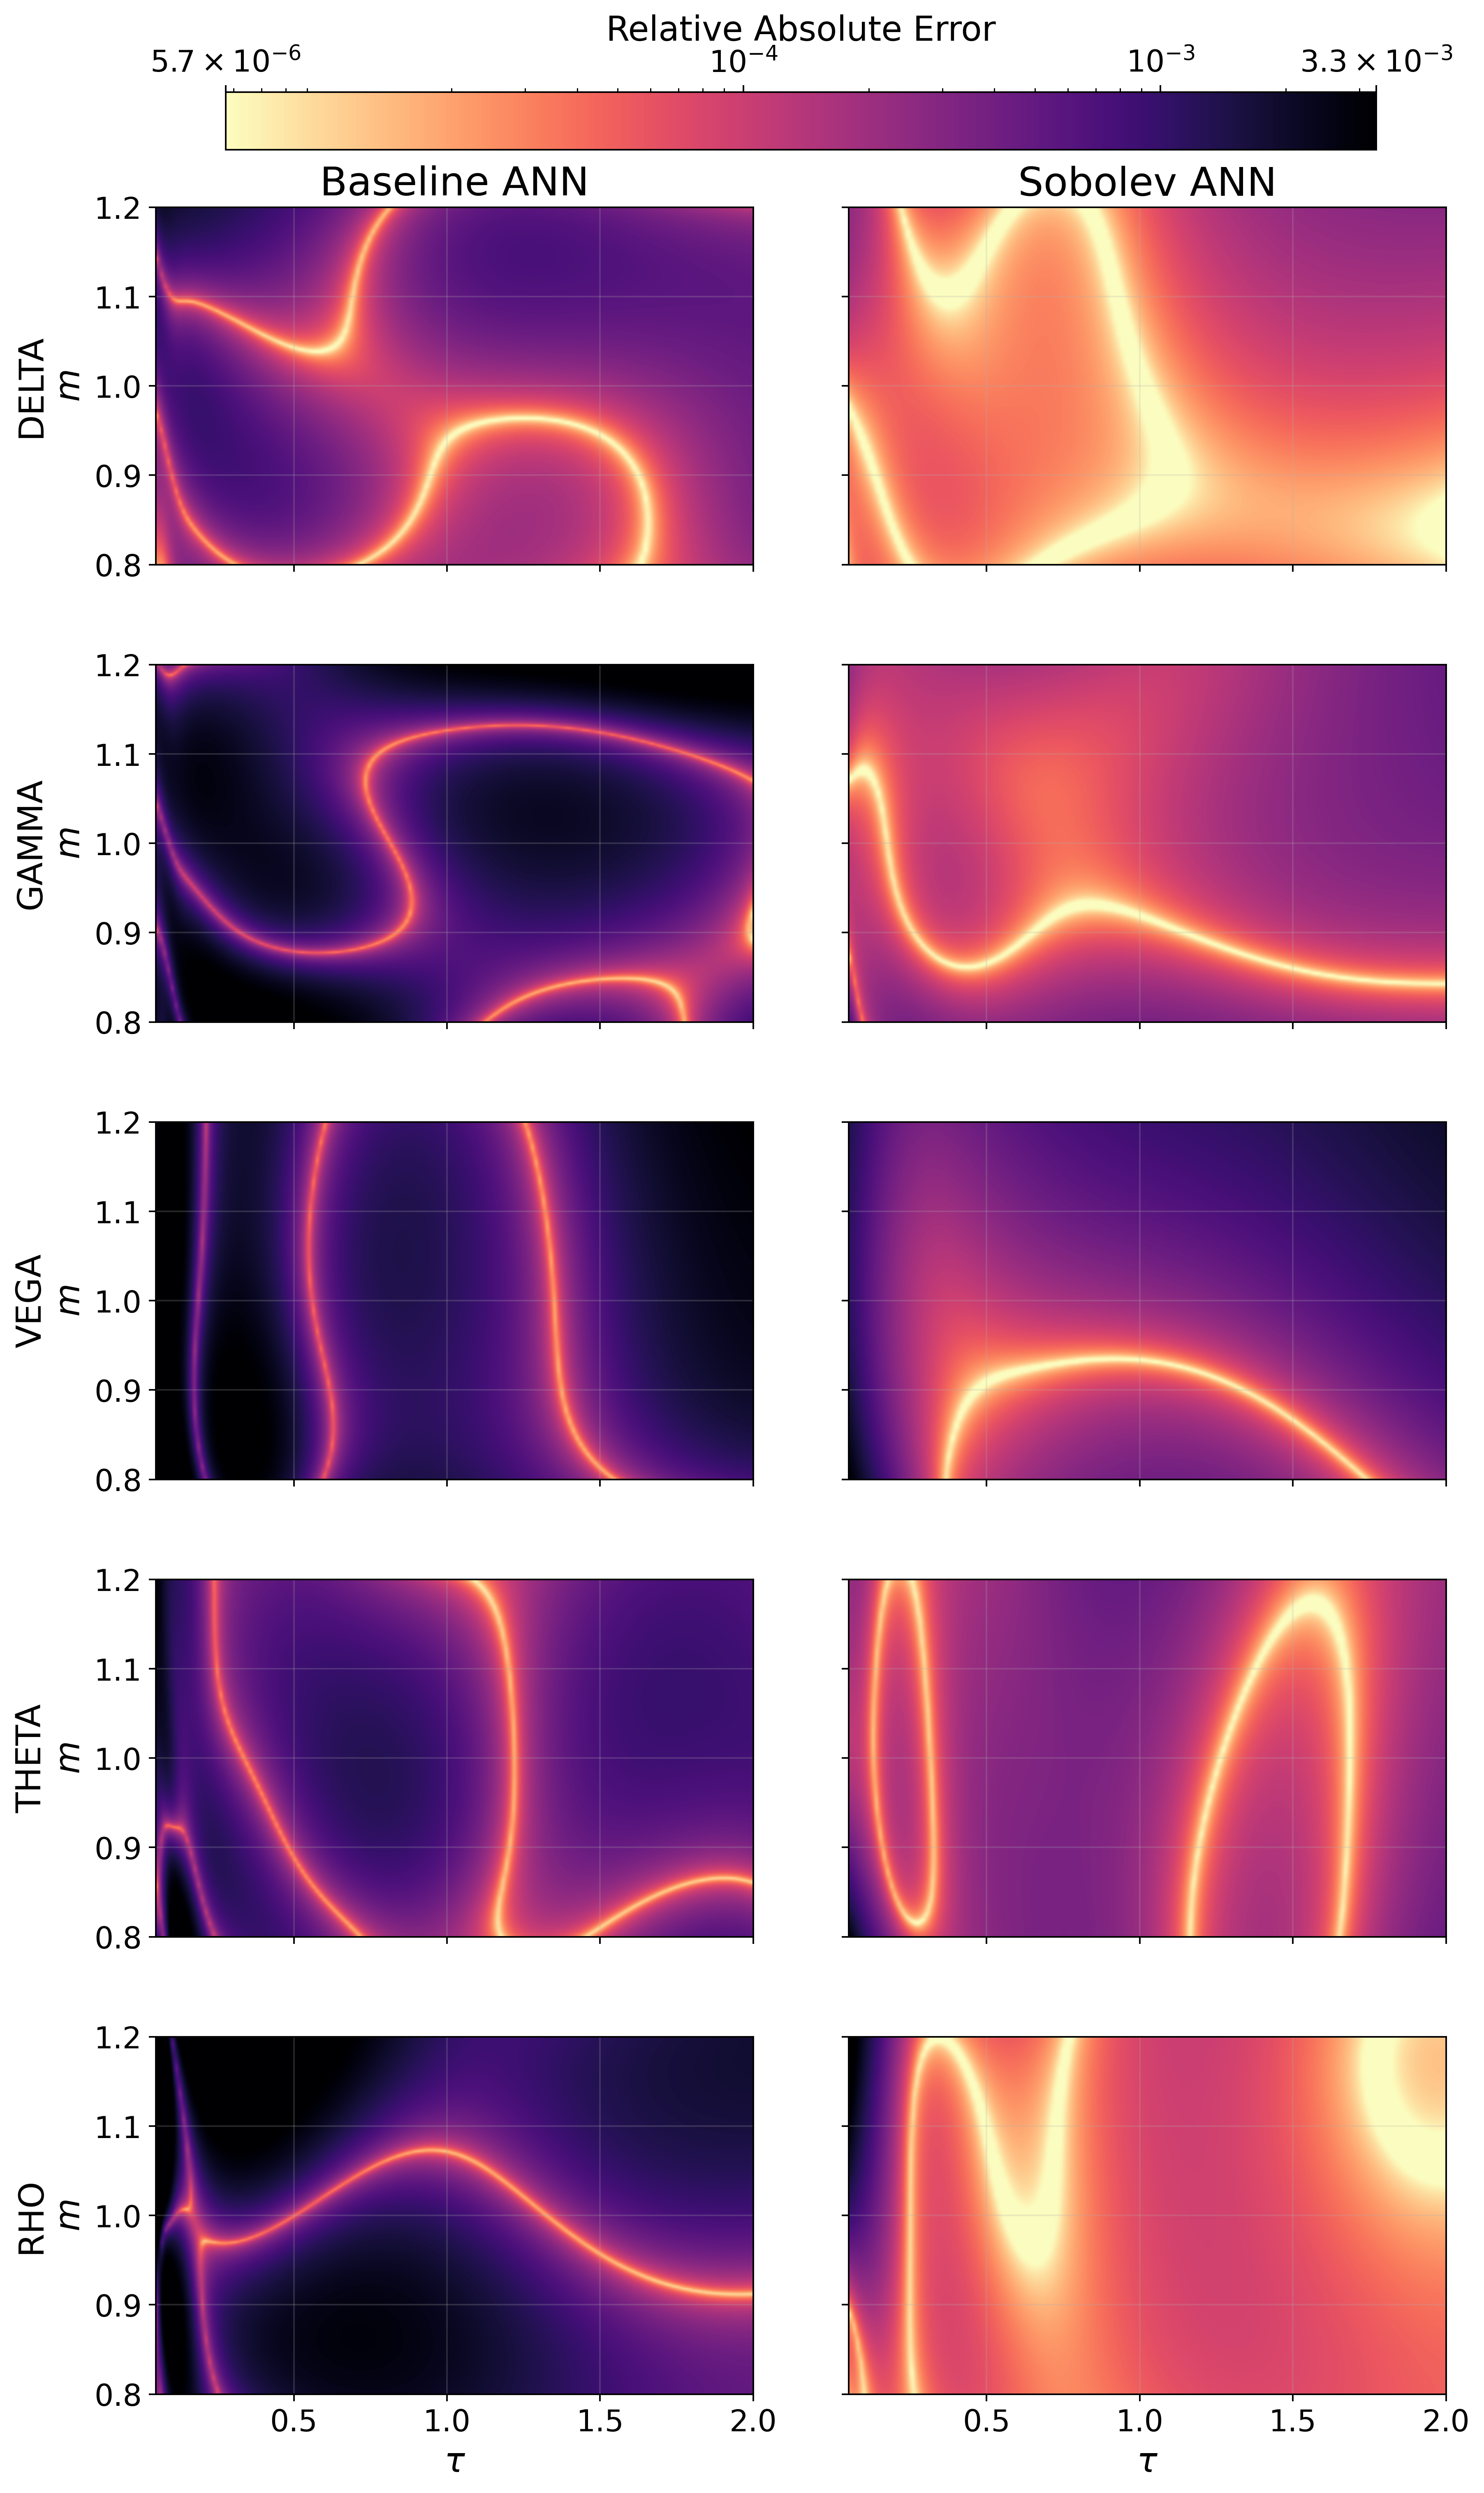
\includegraphics[width=0.90\textwidth]{figures/nn/ann_iv_baseline_vs_sobolev_rel_error_maps_10panel.png}
    \caption{Relative absolute-error maps for ANN-derived Greeks. For each Greek, the baseline ANN and the ANN Sobolev surrogate are evaluated on the same fixed \((m,\tau)\) grid against the Heston characteristic-function reference. Sobolev training visibly contracts the high-error regions and gives a more homogeneous sensitivity surface, especially for GAMMA, RHO, and DELTA.}
    \label{fig:ann_baseline_sobolev_greek_rel_error_maps}
\end{figure}

\subsection{CaNN: Calibration With The ANN Surrogate}
\label{sec:cann_performance}
This section reports the benchmark outcomes of the CaNN workflow after the ANN baseline and the ANN Sobolev surrogate have been fixed. The compact calibration setup and diagnostic reading are introduced in Section~\ref{sec:cann_inverse_problem}; here we focus on the final calibration metrics and on how the inverse problem changes when the frozen forward evaluator is replaced by the Sobolev-trained ANN.

\subsubsection{Benchmark Snapshot}

The calibration benchmark follows the inverse-problem construction of Section~\ref{sec:cann_setup}. In both cases, CaNN uses a frozen supervised ANN surrogate as fast implied-volatility evaluator and calibrates the vector \((\rho,\kappa,\gamma,\bar v,v_0)\) from one fixed quote universe of 35 contracts (Table~\ref{tab:cann_quote_universe}). The comparison is centered on the forward surrogate used inside the inverse loop: the ANN baseline or the ANN Sobolev model. Both calibrations use the same quote grid, the same synthetic truth, the same admissible Heston parameter box, and the same Differential Evolution plus local-polish strategy, with the final optimizer controls taken from each stored run configuration.

\begin{table}[H]
    \ttabbox[\FBwidth]
    {\caption{Quote universe used in the CaNN benchmark.}\label{tab:cann_quote_universe}}
    {\begin{tabular}{|P{4.2cm}|P{6.9cm}|}
        \hline
        \textbf{Item} & \textbf{Value} \\
        \hline
        Number of quotes & 35 \\
        \hline
        Grid structure & Complete \(5\times7\) grid over \((m,\tau)\) \\
        \hline
        Moneyness nodes \(m\) & \(\{0.85,0.925,1.00,1.075,1.15\}\) \\
        \hline
        Maturity nodes \(\tau\) & \(\{0.50,0.75,1.00,1.25,1.50,1.75,2.00\}\) \\
        \hline
        Interest rate \(r\) & 0.03 (constant across quotes) \\
        \hline
        \multicolumn{2}{l}{Source: Own elaboration}
    \end{tabular}}
\end{table}

\subsubsection{Fit Quality And Convergence}

Table~\ref{tab:cann_residual_distribution} reports quote-level calibration residuals in implied-volatility units for the two CaNN variants. The residual is defined as \(e=\hat\sigma_{\mathrm{IV}}-\sigma_{\mathrm{IV}}^{\mathrm{mkt}}\) on the fixed \(35\)-quote Liu grid. The table does not include Liu et al. because the reference paper reports the weighted objective and parameter errors used in Table~\ref{tab:cann_vs_liu}, but not the same quote-level RMSE and MAPE decomposition.

\begin{table}[H]
    \ttabbox[\FBwidth]
    {\caption{CaNN calibration fit.}\label{tab:cann_residual_distribution}}
    {\small
    \begin{tabular}{|P{2.7cm}|P{1.1cm}|P{2.15cm}|P{2.15cm}|P{1.8cm}|P{1.8cm}|}
        \hline
        \textbf{Forward surrogate} & \(\mathbf{n}\) & \textbf{MSE} & \textbf{RMSE} & \textbf{MAPE (\%)} & \(\mathbf{\max |e|}\) \\
        \hline
        ANN baseline & 35 & \(7.43\times10^{-10}\) & \(2.73\times10^{-5}\) & 0.0048 & \(6.79\times10^{-5}\) \\
        \hline
        ANN Sobolev & 35 & \(3.69\times10^{-11}\) & \(6.08\times10^{-6}\) & 0.0011 & \(1.36\times10^{-5}\) \\
        \hline
        \multicolumn{6}{l}{Source: Own elaboration from stored quote-level calibration outputs}
    \end{tabular}}
\end{table}

The Sobolev surrogate gives the tighter quote fit: the residual RMSE falls from \(2.73\times10^{-5}\) to \(6.08\times10^{-6}\), and the maximum absolute residual is reduced by roughly a factor of five. The MAPE values are very small in both cases because the replicated Liu grid is smooth and remains inside the interpolation region, but the same ordering is preserved in relative terms. This suggests that the Sobolev information does not only improve derivative diagnostics later in the ANN branch; in this controlled calibration problem it also makes the inverse fit more precise in IV space.

\subsubsection{Parameter Recovery Profile}

Since this quote set includes sidecar synthetic truth, parameter-level errors can be reported directly. Table~\ref{tab:cann_vs_liu} compares both CaNN variants with the Liu et al. reference values.

\begin{table}[H]
    \ttabbox[\FBwidth]
    {\caption{CaNN calibration results using ANN baseline and ANN Sobolev surrogates versus Liu et al.}\label{tab:cann_vs_liu}}
    {\small
    \begin{tabular}{|P{2.8cm}|P{2.6cm}|P{2.6cm}|P{2.4cm}|}
        \hline
        \textbf{Metric} & \textbf{CaNN ANN baseline} & \textbf{CaNN ANN Sobolev} & \textbf{Liu et al. \cite{liu}} \\
        \hline
        Weighted MSE & \(7.43\times10^{-10}\) & \(3.69\times10^{-11}\) & \(\sim 10^{-8}\) \\
        \hline
        \(|\rho-\rho^\star|\) & \(8.05\times10^{-3}\) & \(1.79\times10^{-3}\) & \(4.84\times10^{-2}\) \\
        \hline
        \(|\kappa-\kappa^\star|\) & \(8.48\times10^{-4}\) & \(8.36\times10^{-3}\) & \(4.88\times10^{-2}\) \\
        \hline
        \(|\gamma-\gamma^\star|\) & \(6.57\times10^{-3}\) & \(2.40\times10^{-3}\) & \(3.28\times10^{-2}\) \\
        \hline
        \(|\bar v-\bar v^\star|\) & \(1.02\times10^{-4}\) & \(3.08\times10^{-5}\) & \(4.54\times10^{-3}\) \\
        \hline
        \(|v_0-v_0^\star|\) & \(1.83\times10^{-4}\) & \(8.03\times10^{-5}\) & \(4.39\times10^{-4}\) \\
        \hline
        \multicolumn{4}{l}{Source: Own elaboration based on selected run outputs and \cite{liu}.}
    \end{tabular}}
\end{table}

In Table~\ref{tab:cann_vs_liu}, \textit{Weighted MSE} denotes the weighted mean-squared IV residual used as calibration objective. Both CaNN variants improve the Liu et al. reference values on the replicated \(35\)-quote grid. The Sobolev surrogate gives the lowest quote residual and improves four of the five parameter errors relative to the ANN baseline, especially for \(\rho\), \(\gamma\), \(\bar v\), and \(v_0\). The exception is \(\kappa\), where the baseline ANN remains closer to the synthetic truth. Therefore, the Sobolev calibration is retained as the main CaNN result, while the baseline calibration remains useful as a reference showing that the improvement is not only due to the inverse optimizer but also to the forward surrogate used inside it.

\subsubsection{Local Smoothness And Curvature Study}

To characterize local identifiability around the calibrated optimum, Jacobian and Hessian diagnostics were computed at \(\theta^\star\) for both CaNN variants. In Table~\ref{tab:cann_hessian_diagnostics}, \(\mathrm{cond}_{\mathrm{abs}}(H)\) denotes the absolute Hessian condition number, computed as the ratio between the largest and smallest absolute eigenvalues. A large value indicates local ill-conditioning: small changes along some parameter directions are weakly penalized compared with others, so the inverse problem is less stable in those directions.

\begin{table}[H]
    \ttabbox[\FBwidth]
    {\caption{CaNN local curvature.}\label{tab:cann_hessian_diagnostics}}
    {\small
    \begin{tabular}{|P{1.8cm}|P{2.0cm}|P{2.25cm}|P{1.8cm}|P{1.8cm}|P{2.2cm}|}
        \hline
        Variant & \(J(\theta^\star)\) & \(\|\nabla J(\theta^\star)\|_2\) & \(\lambda_{\min}(H)\) & \(\lambda_{\max}(H)\) & \(\mathrm{cond}_{\mathrm{abs}}(H)\) \\
        \hline
        ANN baseline & \(2.60\cdot10^{-8}\) & \(1.24\cdot10^{-5}\) & \(4.67\cdot10^{-5}\) & \(41.8\) & \(8.93\cdot10^{5}\) \\
        \hline
        ANN Sobolev & \(1.31\cdot10^{-9}\) & \(2.28\cdot10^{-6}\) & \(4.56\cdot10^{-5}\) & \(42.0\) & \(9.20\cdot10^{5}\) \\
        \hline
        \multicolumn{6}{l}{Source: Own elaboration}
    \end{tabular}}
\end{table}

Table~\ref{tab:cann_hessian_diagnostics} separates two effects. The Sobolev surrogate gives a much smaller objective value and a smaller gradient norm at the calibrated point, so the retained solution is closer to first-order stationarity. However, the extreme Hessian eigenvalues and \(\mathrm{cond}_{\mathrm{abs}}(H)\) remain almost unchanged. Therefore, this curvature diagnostic should not be interpreted as the main source of the Sobolev improvement; it mainly reflects the local geometry of the same 35-quote inverse problem.

To make the matrix-level reading explicit, Table~\ref{tab:cann_sobolev_hessian_matrix} reports the Hessian \(H=\nabla^2J(\theta^\star)\) for the retained Sobolev CaNN run.

\begin{table}[H]
    \ttabbox[\FBwidth]
    {\caption{CaNN Sobolev Hessian.}\label{tab:cann_sobolev_hessian_matrix}}
    {\footnotesize
    \begin{tabular}{|P{1.3cm}|P{1.95cm}|P{1.95cm}|P{1.95cm}|P{1.95cm}|P{1.95cm}|}
        \hline
        & \(\rho\) & \(\kappa\) & \(\gamma\) & \(\bar v\) & \(v_0\) \\
        \hline
        \(\rho\) & \(2.55\cdot10^{-2}\) & \(2.91\cdot10^{-3}\) & \(-6.33\cdot10^{-2}\) & \(0.429\) & \(0.525\) \\
        \hline
        \(\kappa\) & \(2.91\cdot10^{-3}\) & \(6.45\cdot10^{-4}\) & \(-5.68\cdot10^{-3}\) & \(3.55\cdot10^{-2}\) & \(5.89\cdot10^{-3}\) \\
        \hline
        \(\gamma\) & \(-6.33\cdot10^{-2}\) & \(-5.68\cdot10^{-3}\) & \(0.198\) & \(-1.63\) & \(-2.08\) \\
        \hline
        \(\bar v\) & \(0.429\) & \(3.55\cdot10^{-2}\) & \(-1.63\) & \(15.2\) & \(18.6\) \\
        \hline
        \(v_0\) & \(0.525\) & \(5.89\cdot10^{-3}\) & \(-2.08\) & \(18.6\) & \(28.8\) \\
        \hline
        \multicolumn{6}{l}{Source: Own elaboration}
    \end{tabular}}
\end{table}

Table~\ref{tab:cann_sobolev_hessian_matrix} shows a block structure centered on \((\bar v,v_0)\). Diagonal terms measure local curvature with respect to each individual parameter, while off-diagonal terms measure local cross-coupling between pairs of parameters. In the Sobolev Hessian, the diagonal entries associated with \(\bar v\) and \(v_0\) are the largest, and their off-diagonal term is also large, which indicates that the objective reacts strongly to movements in this variance block and that both coordinates are locally coupled. By contrast, the \(\kappa\)-related diagonal curvature is much smaller, so perturbations in that direction are less strongly penalized around \(\theta^\star\). This mixed pattern explains why the Sobolev run can deliver a very tight IV fit while \(\kappa\) remains the one parameter where the baseline calibration is closer to the synthetic truth.

These results define the retained CaNN benchmark for the supervised branch: the ANN Sobolev surrogate is used as the final calibration result, and the ANN baseline calibration is kept as the direct Liu-style reference.

%%%%%%%%%%%%%%%%%%%%%%%%%%%%%%%%%%%%%%%%%%%%%%%%%
\section{Unsupervised PINN Benchmarks}
\label{sec:pinn_pricing_performance}
\todos{Reformular como PINN baseline pricing: modelo no supervisado sobre precio, con resultados razonables y rapidos pero no directamente comparables con ANN-IV supervisada.}
This section reports the baseline PINN pricing quality before introducing Sobolev terms in the training objective. The goal is to establish a reproducible reference for price-level accuracy and runtime against the COS/Heston engine.

\subsection{PINN Baseline}

The detailed reproducible setup (input convention, standardization, reference parameters, filtering, and arithmetic context) is moved to Appendix~\ref{app:pinn_pricing_benchmark_setup}. In the final pricing diagnostic used here, the baseline parametric PINN without Sobolev terms is evaluated against the Heston reference on the same fixed grid later used for the Sobolev comparison: \(25\,921\) valid points over \(m\in[0.8,1.2]\) and \(\tau\in[0.05,2.0]\).

\subsubsection{Global Pricing Metrics}

The compact global summary is embedded in Figure~\ref{fig:pinn_pricing_composite}: MSE \(=9.43\times10^{-8}\), RMSE \(=3.07\times10^{-4}\), and MAPE \(=0.28\%\). These results are obtained with the baseline PINN only (without Sobolev augmentation) on the final fixed grid, so they can be read directly against the Sobolev pricing diagnostic in Figure~\ref{fig:pinn_pricing_composite_sobolev}.
\todos{Anadir lectura comparativa de PINN baseline frente a PINN Sobolev y PINN Sobolev+ACV si tambien hay metricas de precio disponibles.}

\subsubsection{Spatial And Distributional Diagnostics}

The pointwise agreement between PINN and reference prices, the global metric table, the spatial error map, and the distributional diagnostic are consolidated in Figure~\ref{fig:pinn_pricing_composite}. The scatter panel is concentrated around the identity line; the more informative panels are therefore the relative-error map and the histogram, which reveal where small price discrepancies become visible after normalization by the reference value.

\begin{figure}[H]
    \centering
    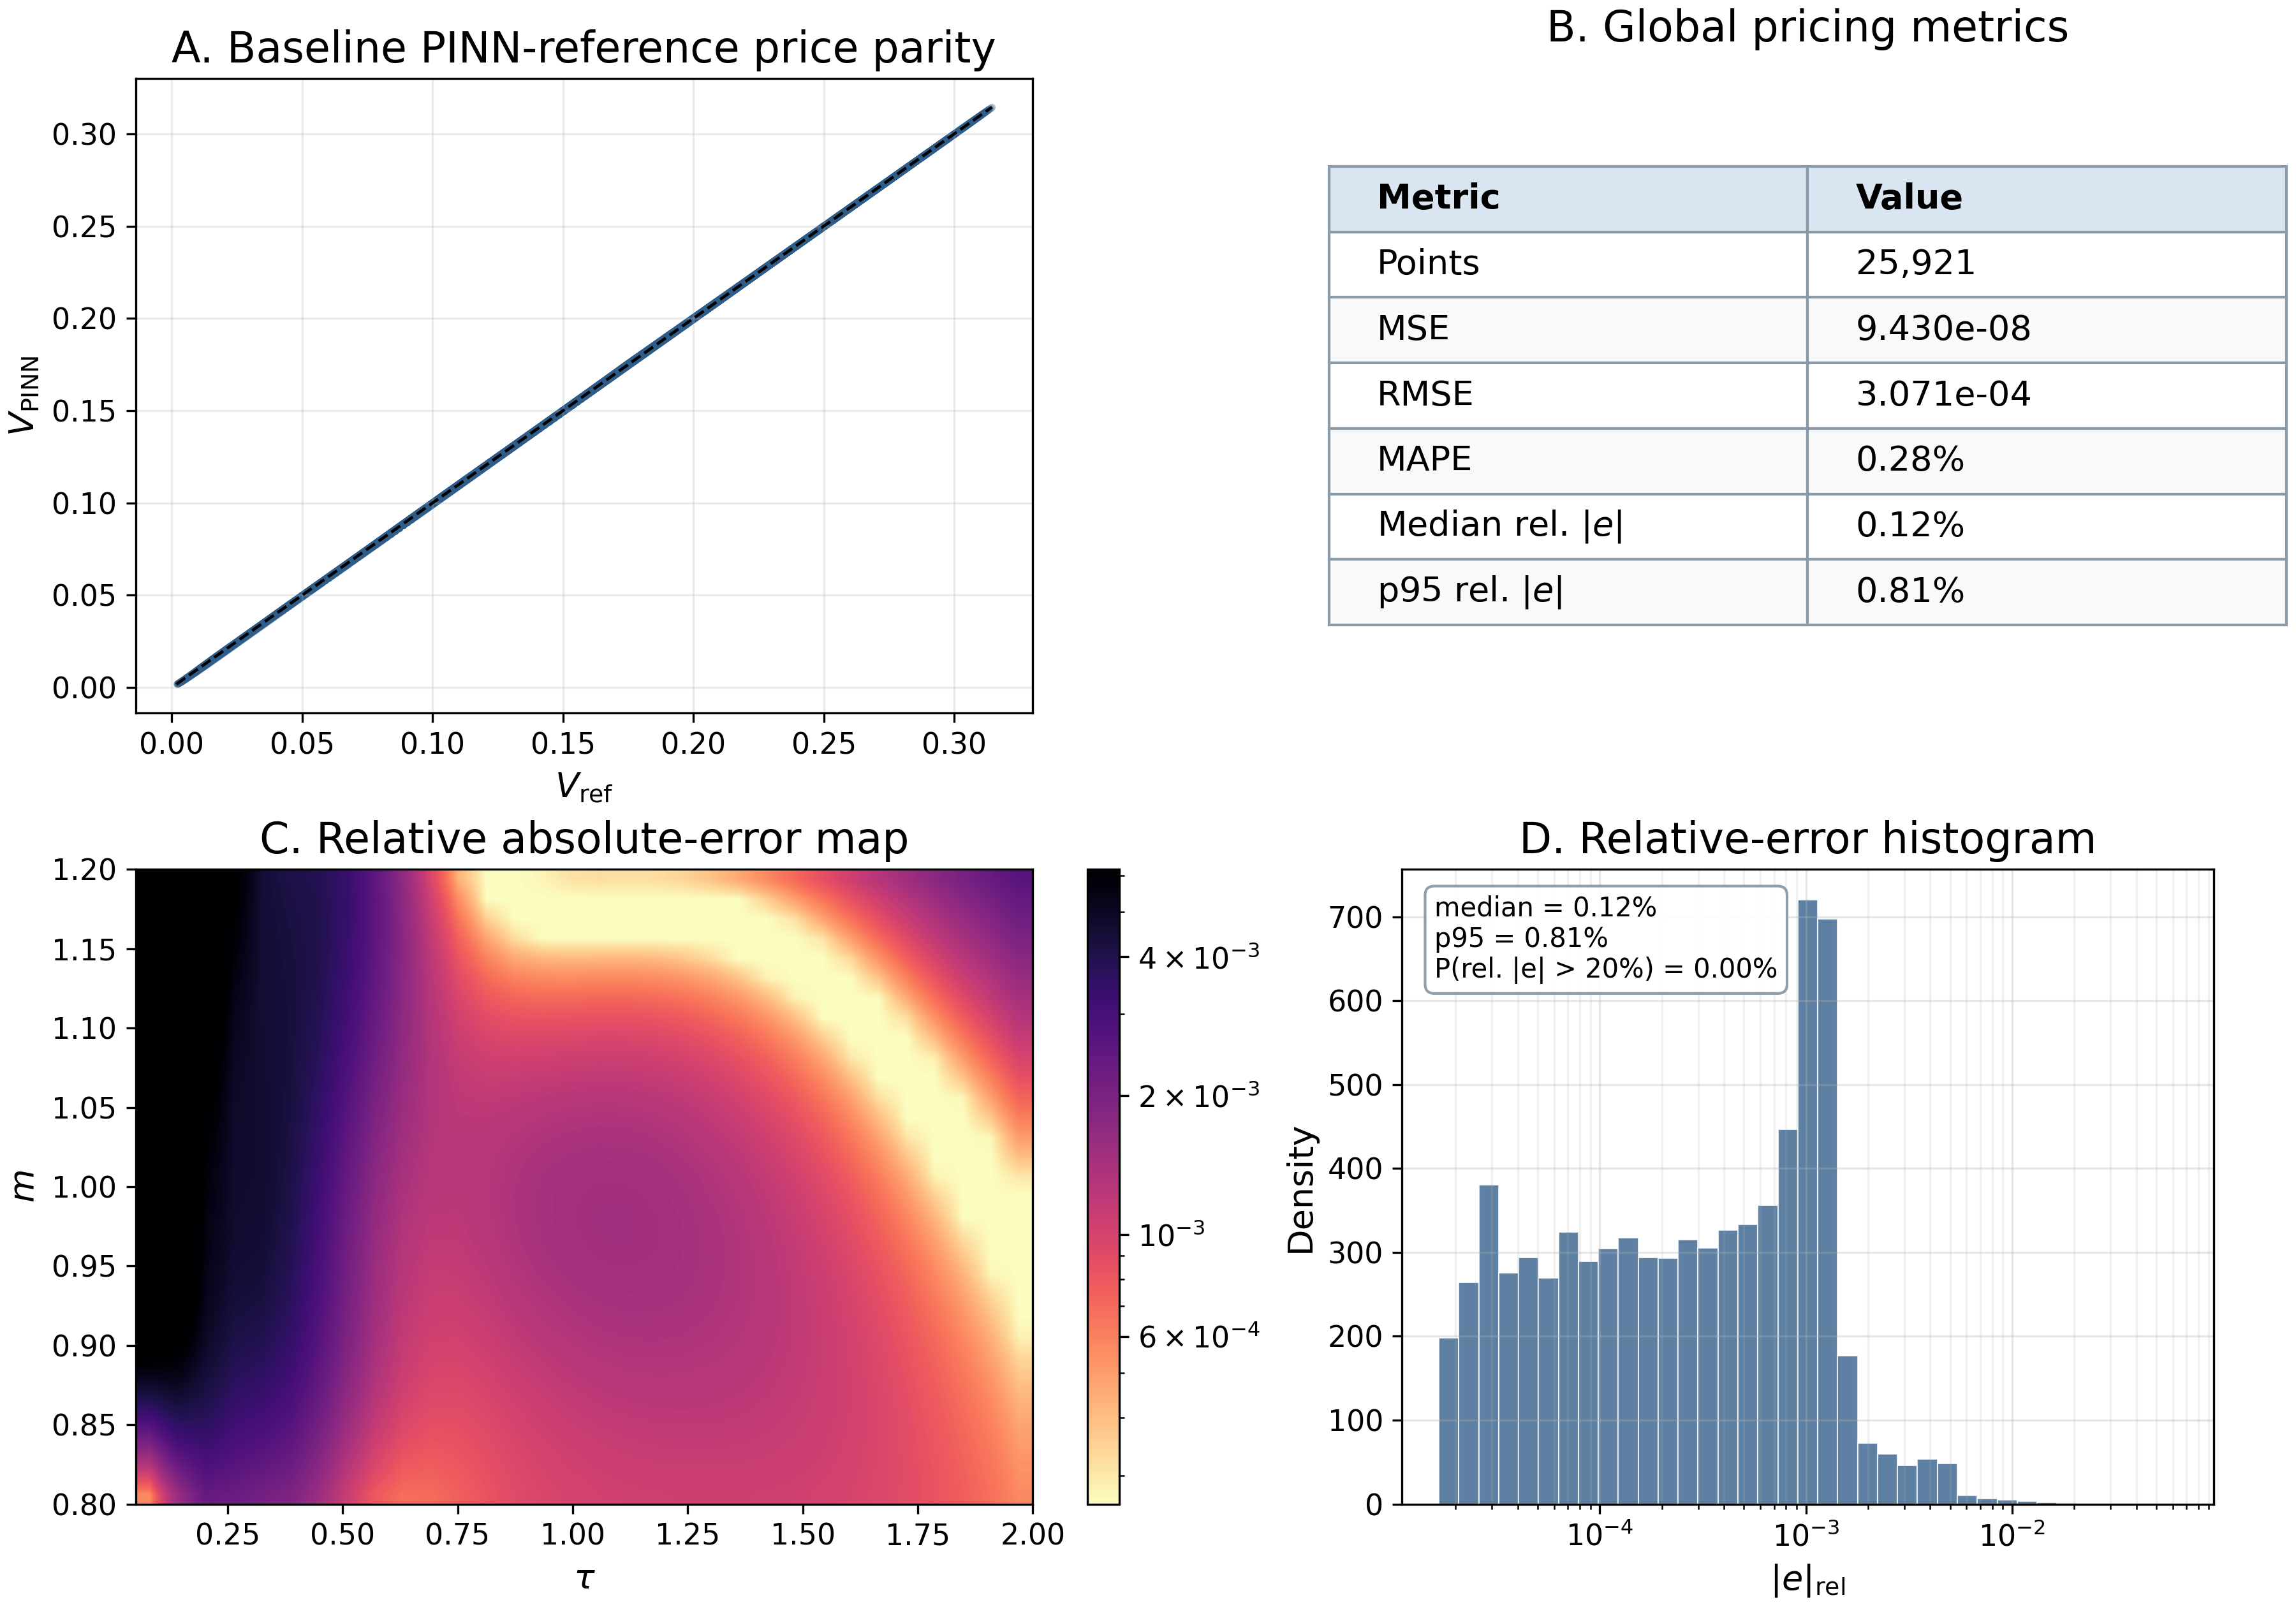
\includegraphics[width=1\textwidth]{figures/pinn/pricing/pricing_benchmark_composite.png}
    \caption[Baseline PINN pricing benchmark versus reference]{Baseline PINN pricing benchmark versus reference. Top-left: PINN-reference scatter. Top-right: global MSE/RMSE/MAPE and relative-error summary. Bottom-left: mean relative absolute-error map over \((\tau,m)\), with the color scale representing the cellwise mean relative absolute error. Bottom-right: histogram of relative absolute pricing errors.}
    \label{fig:pinn_pricing_composite}
\end{figure}

The spatial panel shows that relative error is not homogeneous over \((m,\tau)\). On this common local grid, the largest relative deviations appear near short maturities and in low-reference-price regions, while the central pricing region remains more stable. These values must be interpreted jointly with the absolute-unit metrics (MSE and RMSE): when the reference price is small, relative error can magnify deviations that remain modest in price units. Distributionally, the median relative absolute error is \(0.12\%\), the \(p_{95}\) relative absolute error is \(0.81\%\), and no point exceeds \(20\%\) relative error.

\begin{figure}[H]
    \centering
    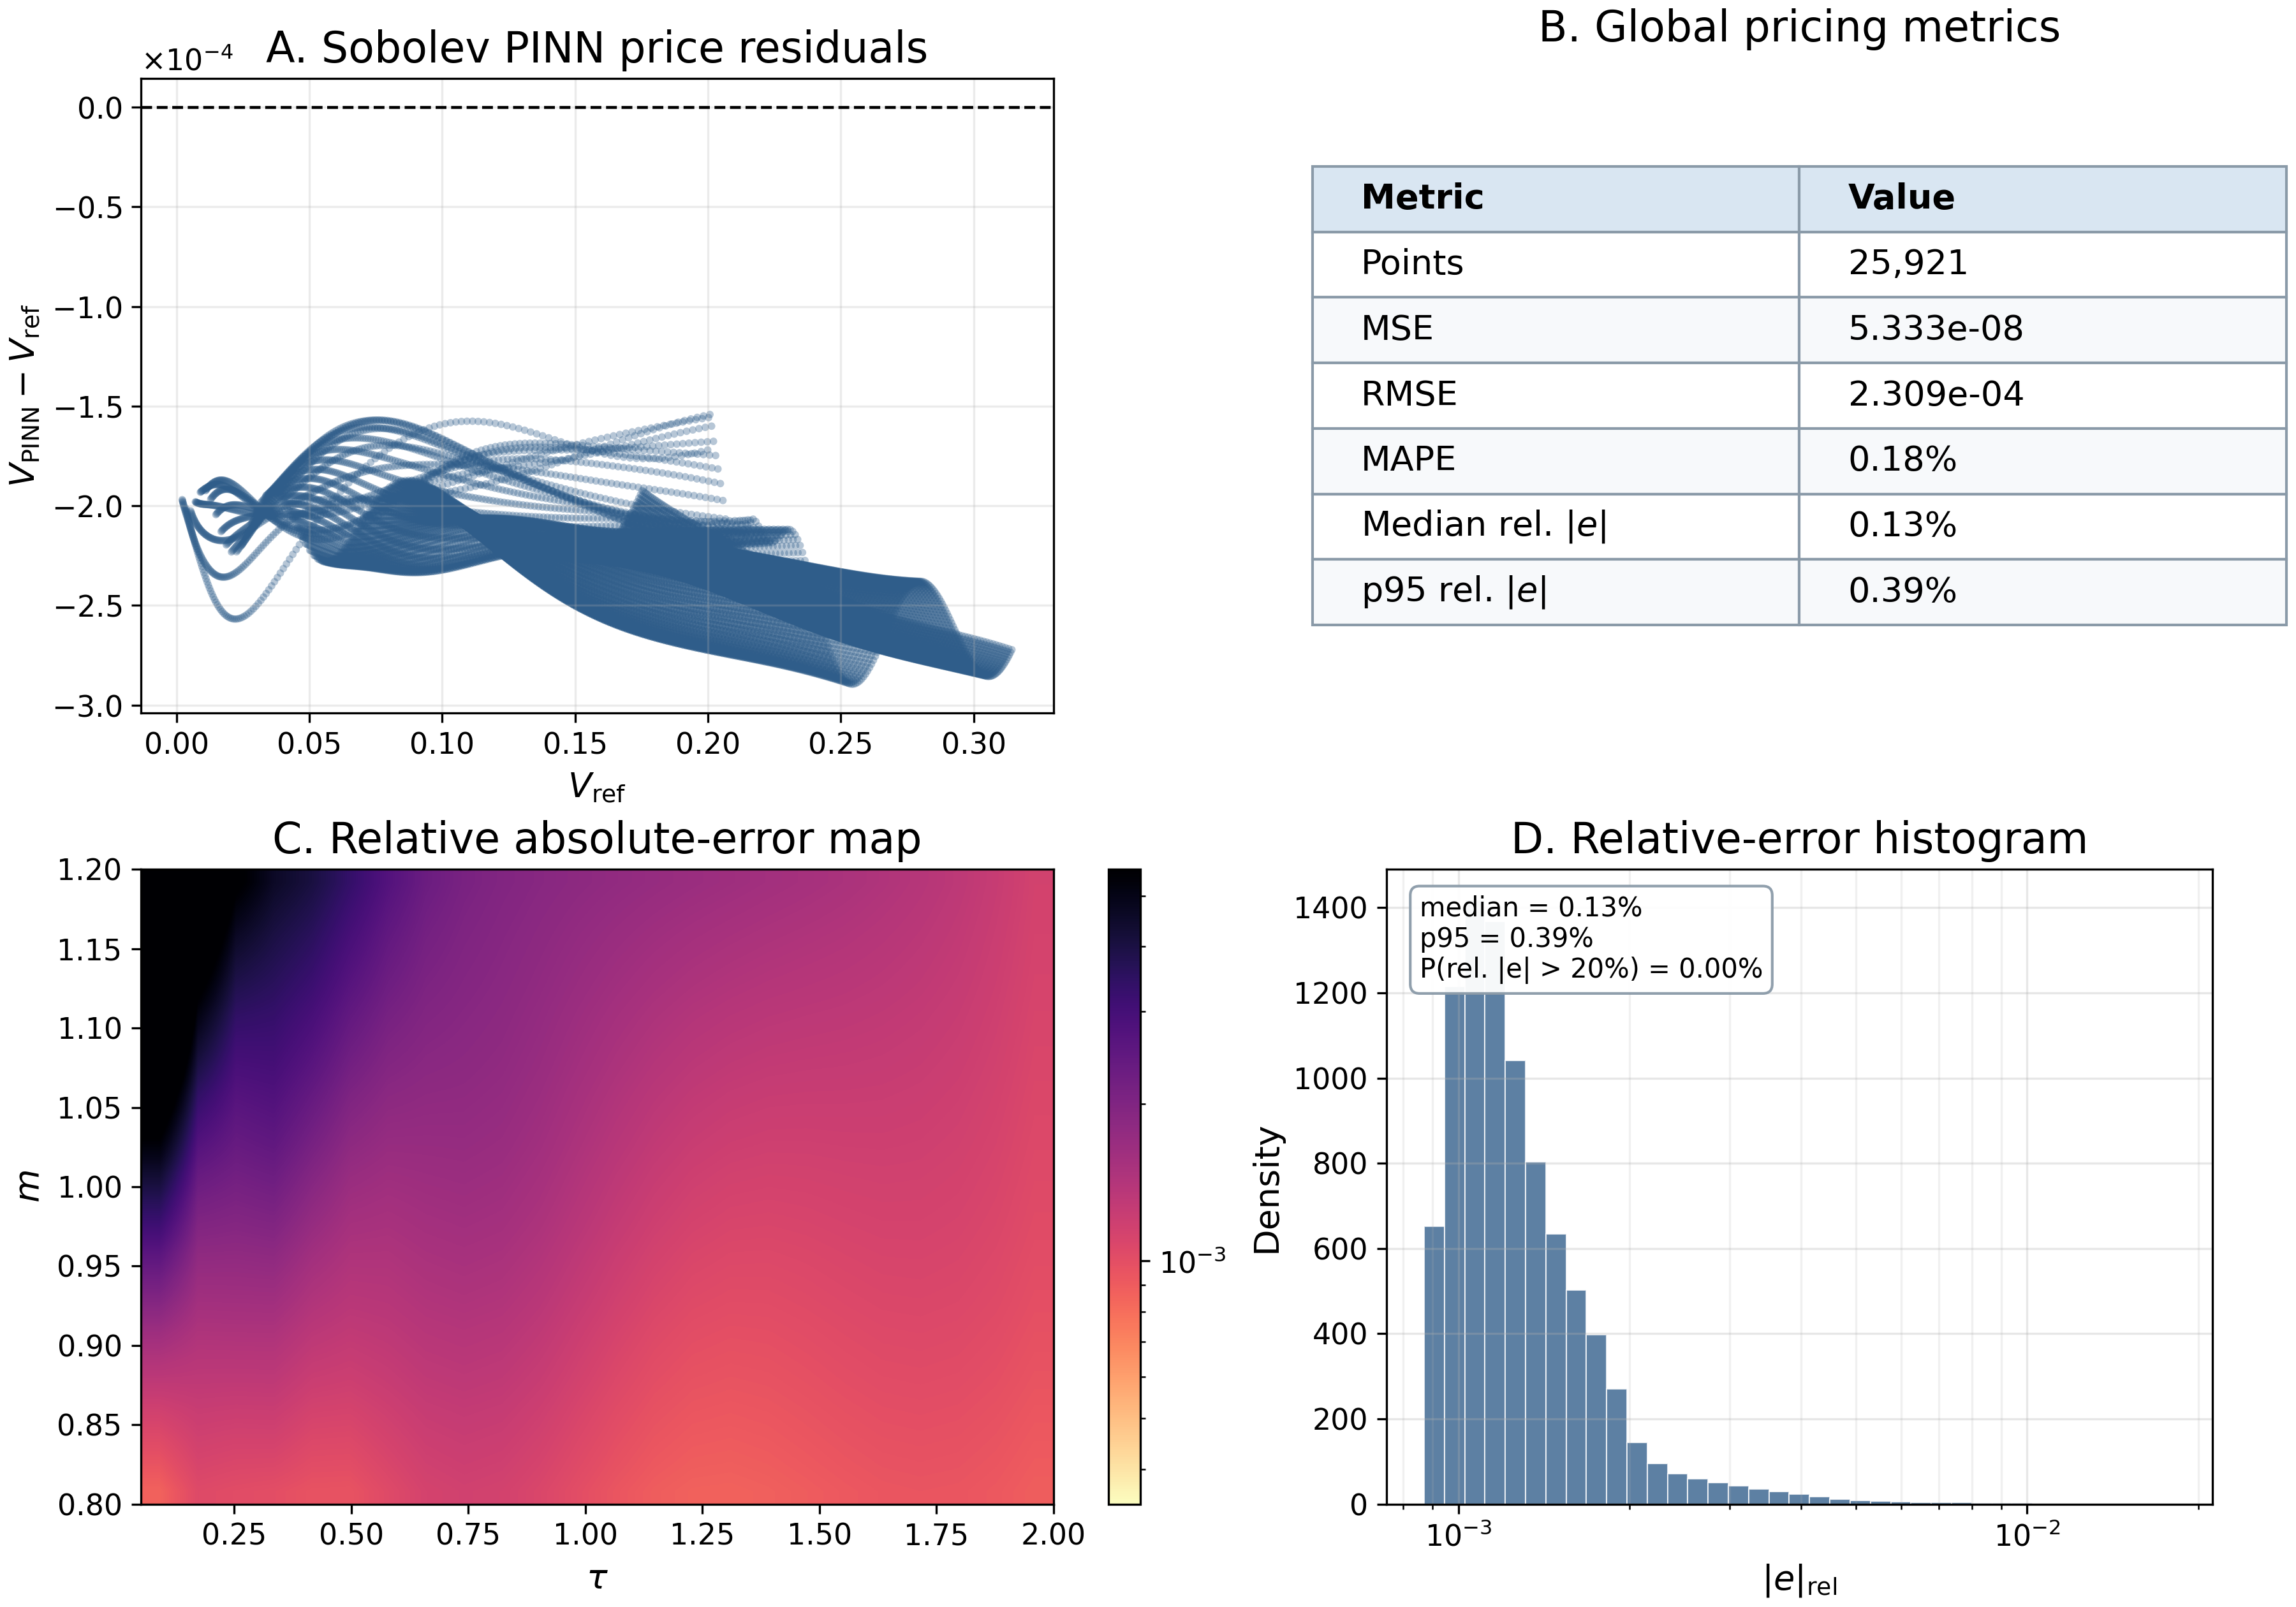
\includegraphics[width=1\textwidth]{figures/pinn/pricing/pricing_benchmark_composite_sobolev_hist.png}
    \caption[Sobolev PINN pricing benchmark versus reference]{ADAPTAR. Sobolev PINN pricing benchmark versus reference. The panels follow the same layout as Figure~\ref{fig:pinn_pricing_composite}; in the spatial panel, the color scale represents the cellwise mean relative absolute error over \((\tau,m)\).}
    \label{fig:pinn_pricing_composite_sobolev}
\end{figure}

\begin{figure}[H]
    \centering
    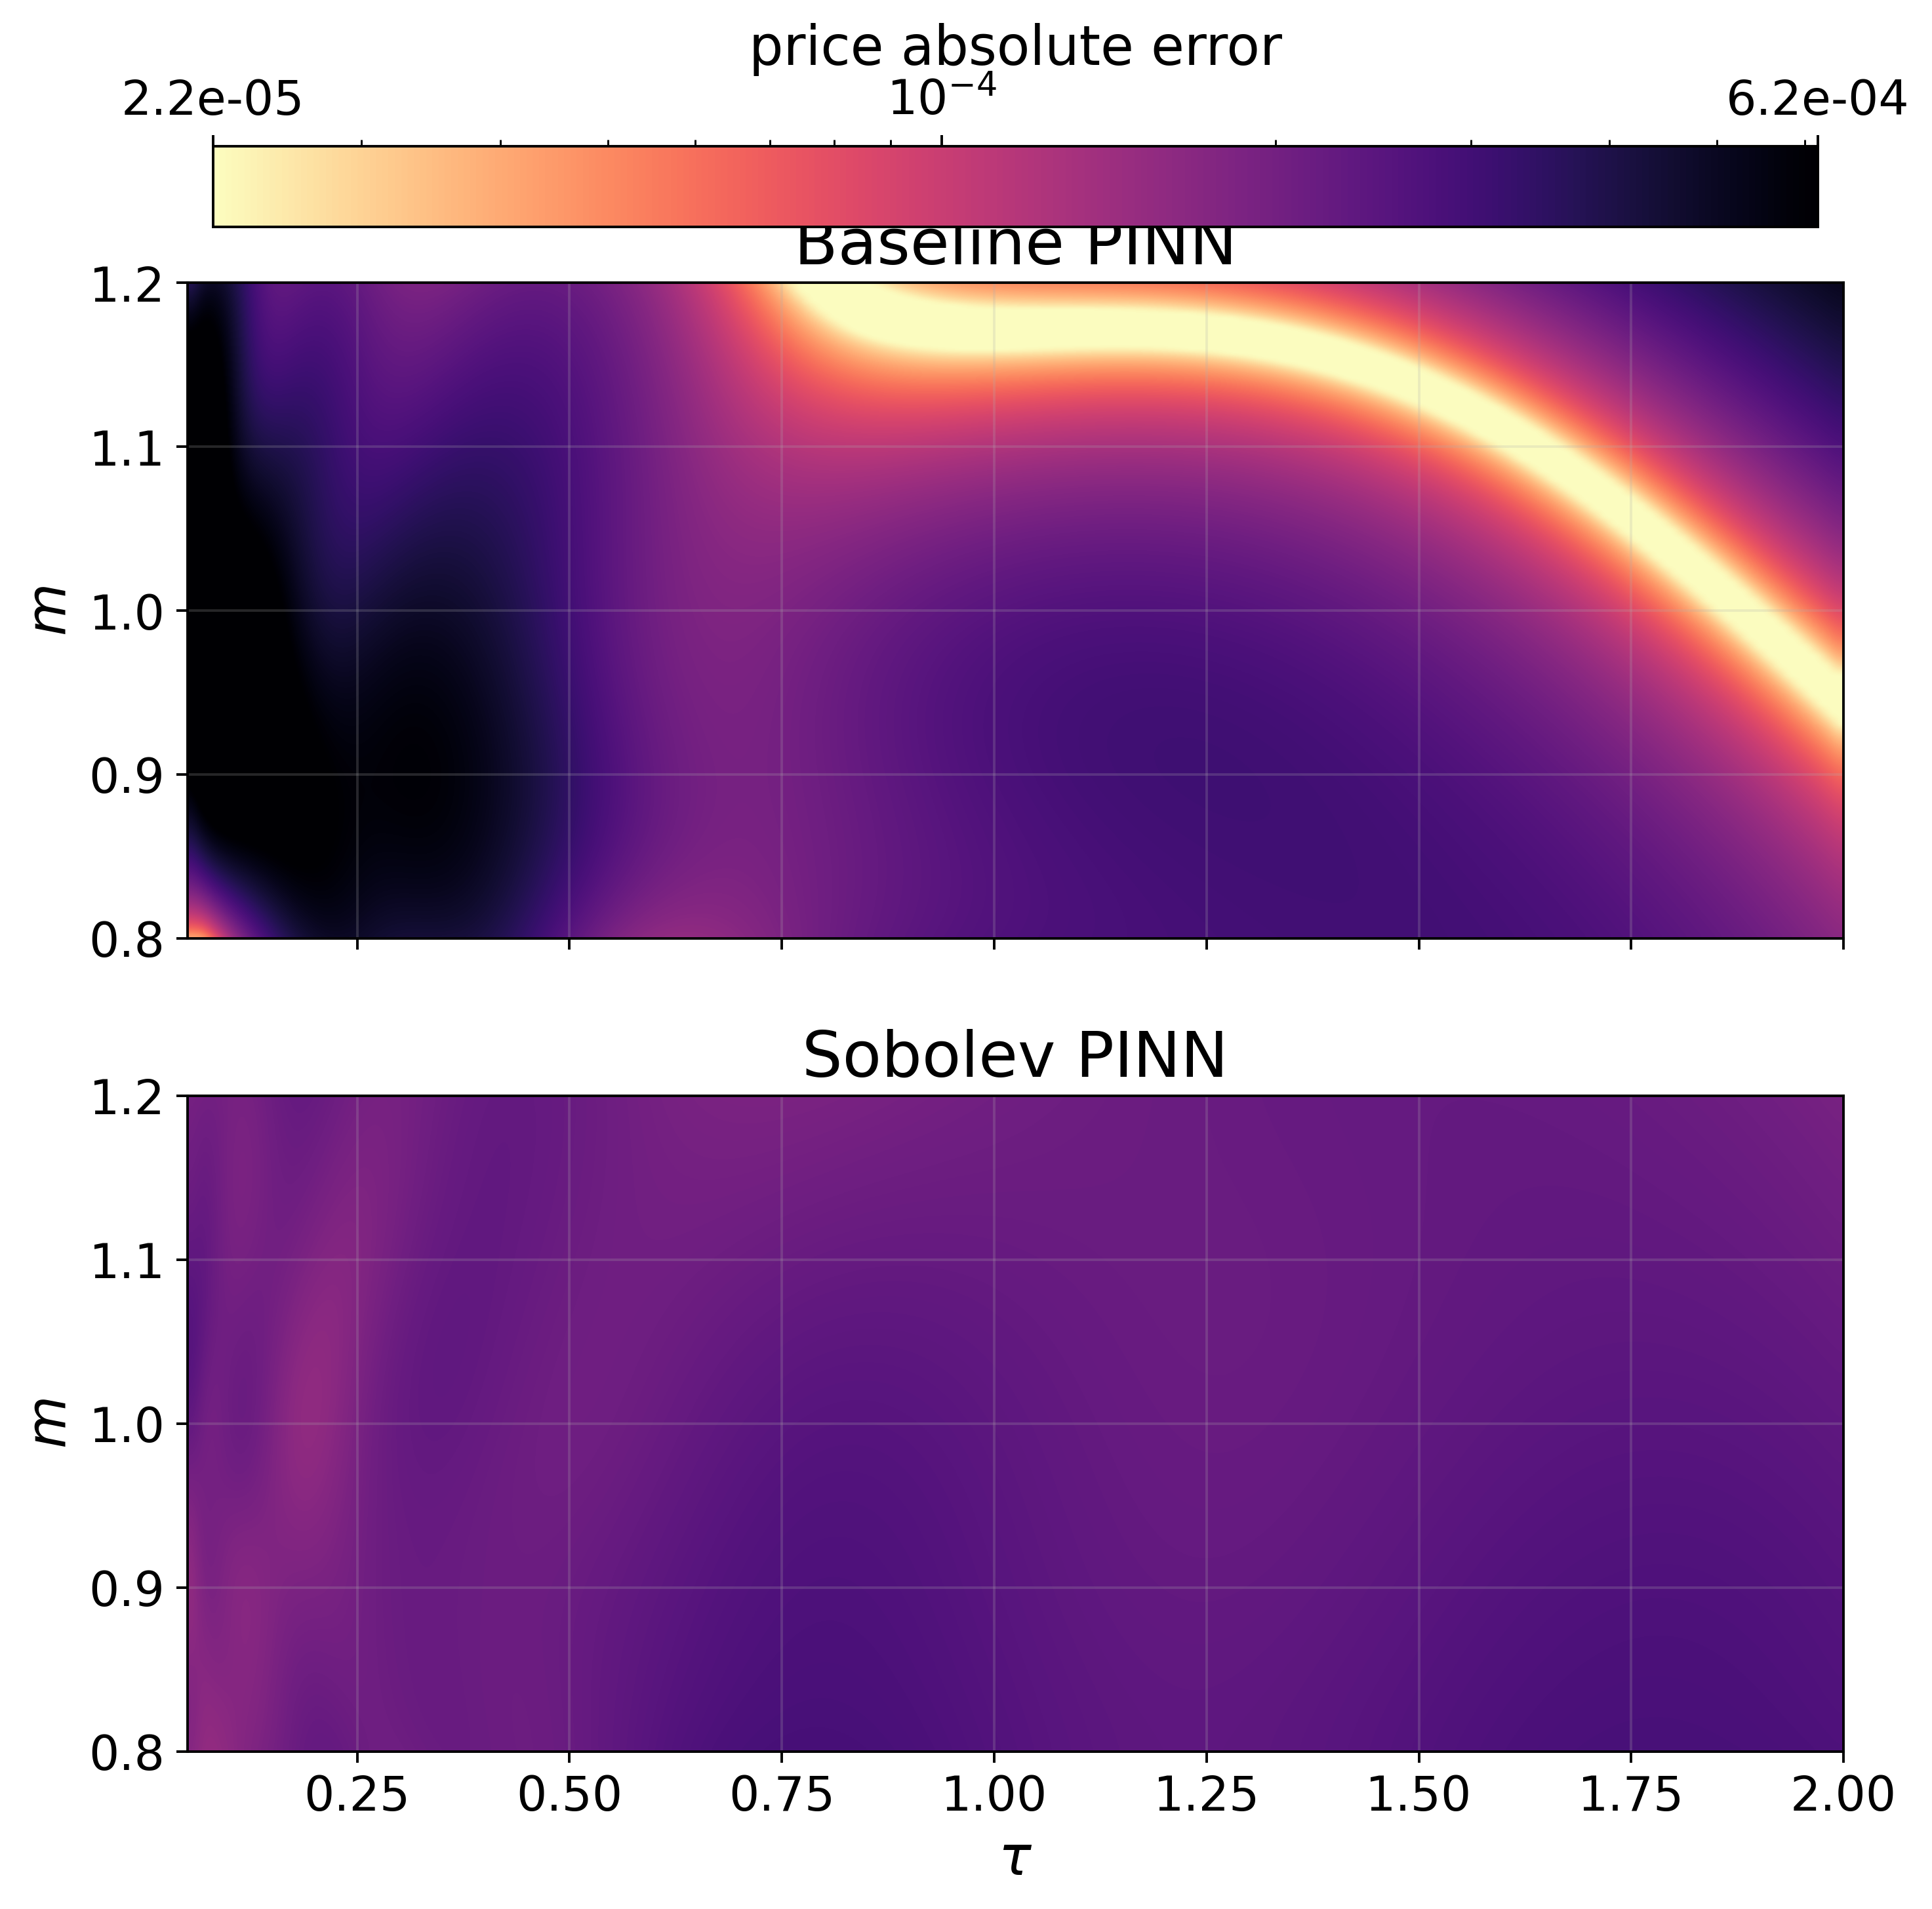
\includegraphics[width=0.88\textwidth]{figures/pinn/pricing/pinn_baseline_sobolev_price_abs_error_maps_2row.png}
    \caption{ADAPTAR}
    \label{fig:pinn_baseline_sobolev_price_abs_error_maps}
\end{figure}

%%%%%%%%%%%%%%%%%%%%%%%%%%%%%%%%%%%%%%%%%%%%%%%%%
\subsection{Sobolev Methods: Greek Improvement And Pricing Trade-Off}
\label{sec:pinn_greeks_performance}
\todos{Separar resultados PINN en tres variantes: PINN baseline, PINN Sobolev y PINN Sobolev+ACV.}
This section evaluates autodiff-based Greek quality for the baseline PINN and quantifies the effect of Sobolev augmentation through a controlled ablation.

\subsubsection{Ablation Design And Reproducible Protocol}
\label{sec:ablation_pinn_sobolev}
The ablation isolates the impact of Jacobian-informed Sobolev terms on top of the baseline PINN objective, comparing:
\todos{Ampliar protocolo para incluir PINN Sobolev+ACV como tercera variante final, no solo baseline vs Sobolev.}
\begin{itemize}
    \item \textbf{Baseline PINN}: PDE + terminal + lower-boundary losses only.
    \item \textbf{Sobolev-augmented PINN}: baseline loss plus derivative supervision terms \(\mathcal{L}_{g,1}\) and \(\mathcal{L}_{g,2}\) as defined in Chapter~\ref{ch:pinn_greeks}.
\end{itemize}

To keep the comparison interpretable, both variants are benchmarked on the same \((m,\tau)\) grid, with identical fixed parameters, the same Heston characteristic-function Greek engine, and the same numerical integration settings.

\begin{table}[H]
    \ttabbox[\FBwidth]
    {\caption{Reproducible protocol for the Greek ablation benchmark.}\label{tab:pinn_greeks_ablation_setup}}
    {\begin{tabular}{|P{4.4cm}|P{6.7cm}|}
        \hline
        \textbf{Item} & \textbf{Value} \\
        \hline
        Compared variants & Baseline PINN vs Sobolev-augmented PINN \\
        \hline
        Architecture and features & Fixed across variants (same parametric PINN input convention) \\
        \hline
        Evaluation grid & \(m\in[0.8,1.2]\) (161 points), \(\tau\in[0.05,2.0]\) (161 points) \\
        \hline
        Total evaluation size & \(n=2.5921\times10^4\) points per Greek \\
        \hline
        Fixed model parameters & \(v=0.04,\ \rho=-0.7,\ \kappa=2.0,\ \gamma=0.3,\ \bar v=0.04,\ r=0.01\) \\
        \hline
        Reference Greeks & Semi-analytical Heston characteristic-function Greeks \\
        \hline
        Characteristic function integration setup & \(u_{\min}=10^{-6}\), \(u_{\max}=200\), \(n_u=1200\) \\
        \hline
        Shared conventions & Put option, strike \(K=1\), THETA sign convention (\(\mathrm{THETA}=-\partial V/\partial\tau\)), MAPE floor \(10^{-4}\) \\
        \hline
        Arithmetic context & Double precision on CPU \\
        \hline
        \multicolumn{2}{l}{Source: Own elaboration}
    \end{tabular}}
\end{table}

\subsubsection{Ablation Metrics By Greek}

Greek quality is reported with the same primary metrics used in the rest of the chapter: MSE, RMSE, and MAPE (\%).
\todos{Actualizar tabla de griegas para incluir PINN Sobolev+ACV y usar nombres finales de modelos.}

\begin{table}[H]
    \ttabbox[\FBwidth]
    {\caption{Greek metrics for baseline and Sobolev PINN (\(n=2.5921\times10^4\) per Greek).}\label{tab:ablation_metrics_by_greek}}
    {\small
    \begin{tabular}{|P{2.0cm}|P{1.7cm}|P{2.0cm}|P{2.0cm}|P{2.0cm}|}
        \hline
        \textbf{Variant} & \textbf{Greek} & \textbf{MSE} & \textbf{RMSE} & \textbf{MAPE (\%)} \\
        \hline
        Baseline & DELTA & \(1.11\times 10^{-3}\) & \(3.33\times 10^{-2}\) & 10.74 \\
        \hline
        Baseline & GAMMA & \(1.48\times 10^{-1}\) & \(3.85\times 10^{-1}\) & 82.98 \\
        \hline
        Baseline & VEGA & \(4.30\times 10^{-3}\) & \(6.55\times 10^{-2}\) & 71.84 \\
        \hline
        Baseline & THETA & \(2.32\times 10^{-5}\) & \(4.82\times 10^{-3}\) & 31.98 \\
        \hline
        Baseline & RHO & \(7.01\times 10^{-3}\) & \(8.37\times 10^{-2}\) & 95.00 \\
        \hline
        Sobolev & DELTA & \(1.23\times 10^{-7}\) & \(3.51\times 10^{-4}\) & 0.28 \\
        \hline
        Sobolev & GAMMA & \(7.99\times 10^{-5}\) & \(8.94\times 10^{-3}\) & 31.29 \\
        \hline
        Sobolev & VEGA & \(1.00\times 10^{-5}\) & \(3.17\times 10^{-3}\) & 36.11 \\
        \hline
        Sobolev & THETA & \(2.81\times 10^{-7}\) & \(5.30\times 10^{-4}\) & 1.88 \\
        \hline
        Sobolev & RHO & \(2.05\times 10^{-6}\) & \(1.43\times 10^{-3}\) & 9.05 \\
        \hline
        \multicolumn{5}{l}{Source: Own elaboration}
    \end{tabular}}
\end{table}

Compared with the baseline PINN, Sobolev augmentation reduces RMSE by approximately \(9\times\) (THETA) to \(95\times\) (DELTA), with the largest practical gains in the previously hardest Greeks (GAMMA and VEGA). Greek-inference throughput decreases from \(9.48\times 10^3\) to \(8.60\times 10^3\) points/s (\(\sim 9.3\%\) reduction), which remains a clearly favorable trade-off given the global accuracy gains.
\todos{Matizar interpretacion: Sobolev-PINN mejora griegas, pero introduce informacion derivativa externa; no venderlo como PINN completamente no supervisada.}

\subsubsection{Visual Diagnostics}

This subsection is organized as a before/after narrative. Baseline diagnostics are first used to localize the dominant Greek-error modes, and Sobolev diagnostics are then read with the same visual layout to make improvements directly comparable.
\todos{Revisar narrativa visual para incluir tambien PINN Sobolev+ACV o dejar claro que estas figuras solo comparan baseline vs Sobolev.}

Figure~\ref{fig:no_sobolev_greeks_error_maps} displays baseline relative absolute-error maps for the five Greeks. The spatial pattern is heterogeneous, with broad high-error regions in GAMMA and VEGA, which is consistent with their weaker baseline MSE/RMSE values in Table~\ref{tab:ablation_metrics_by_greek}.

\begin{figure}[H]
    \centering
    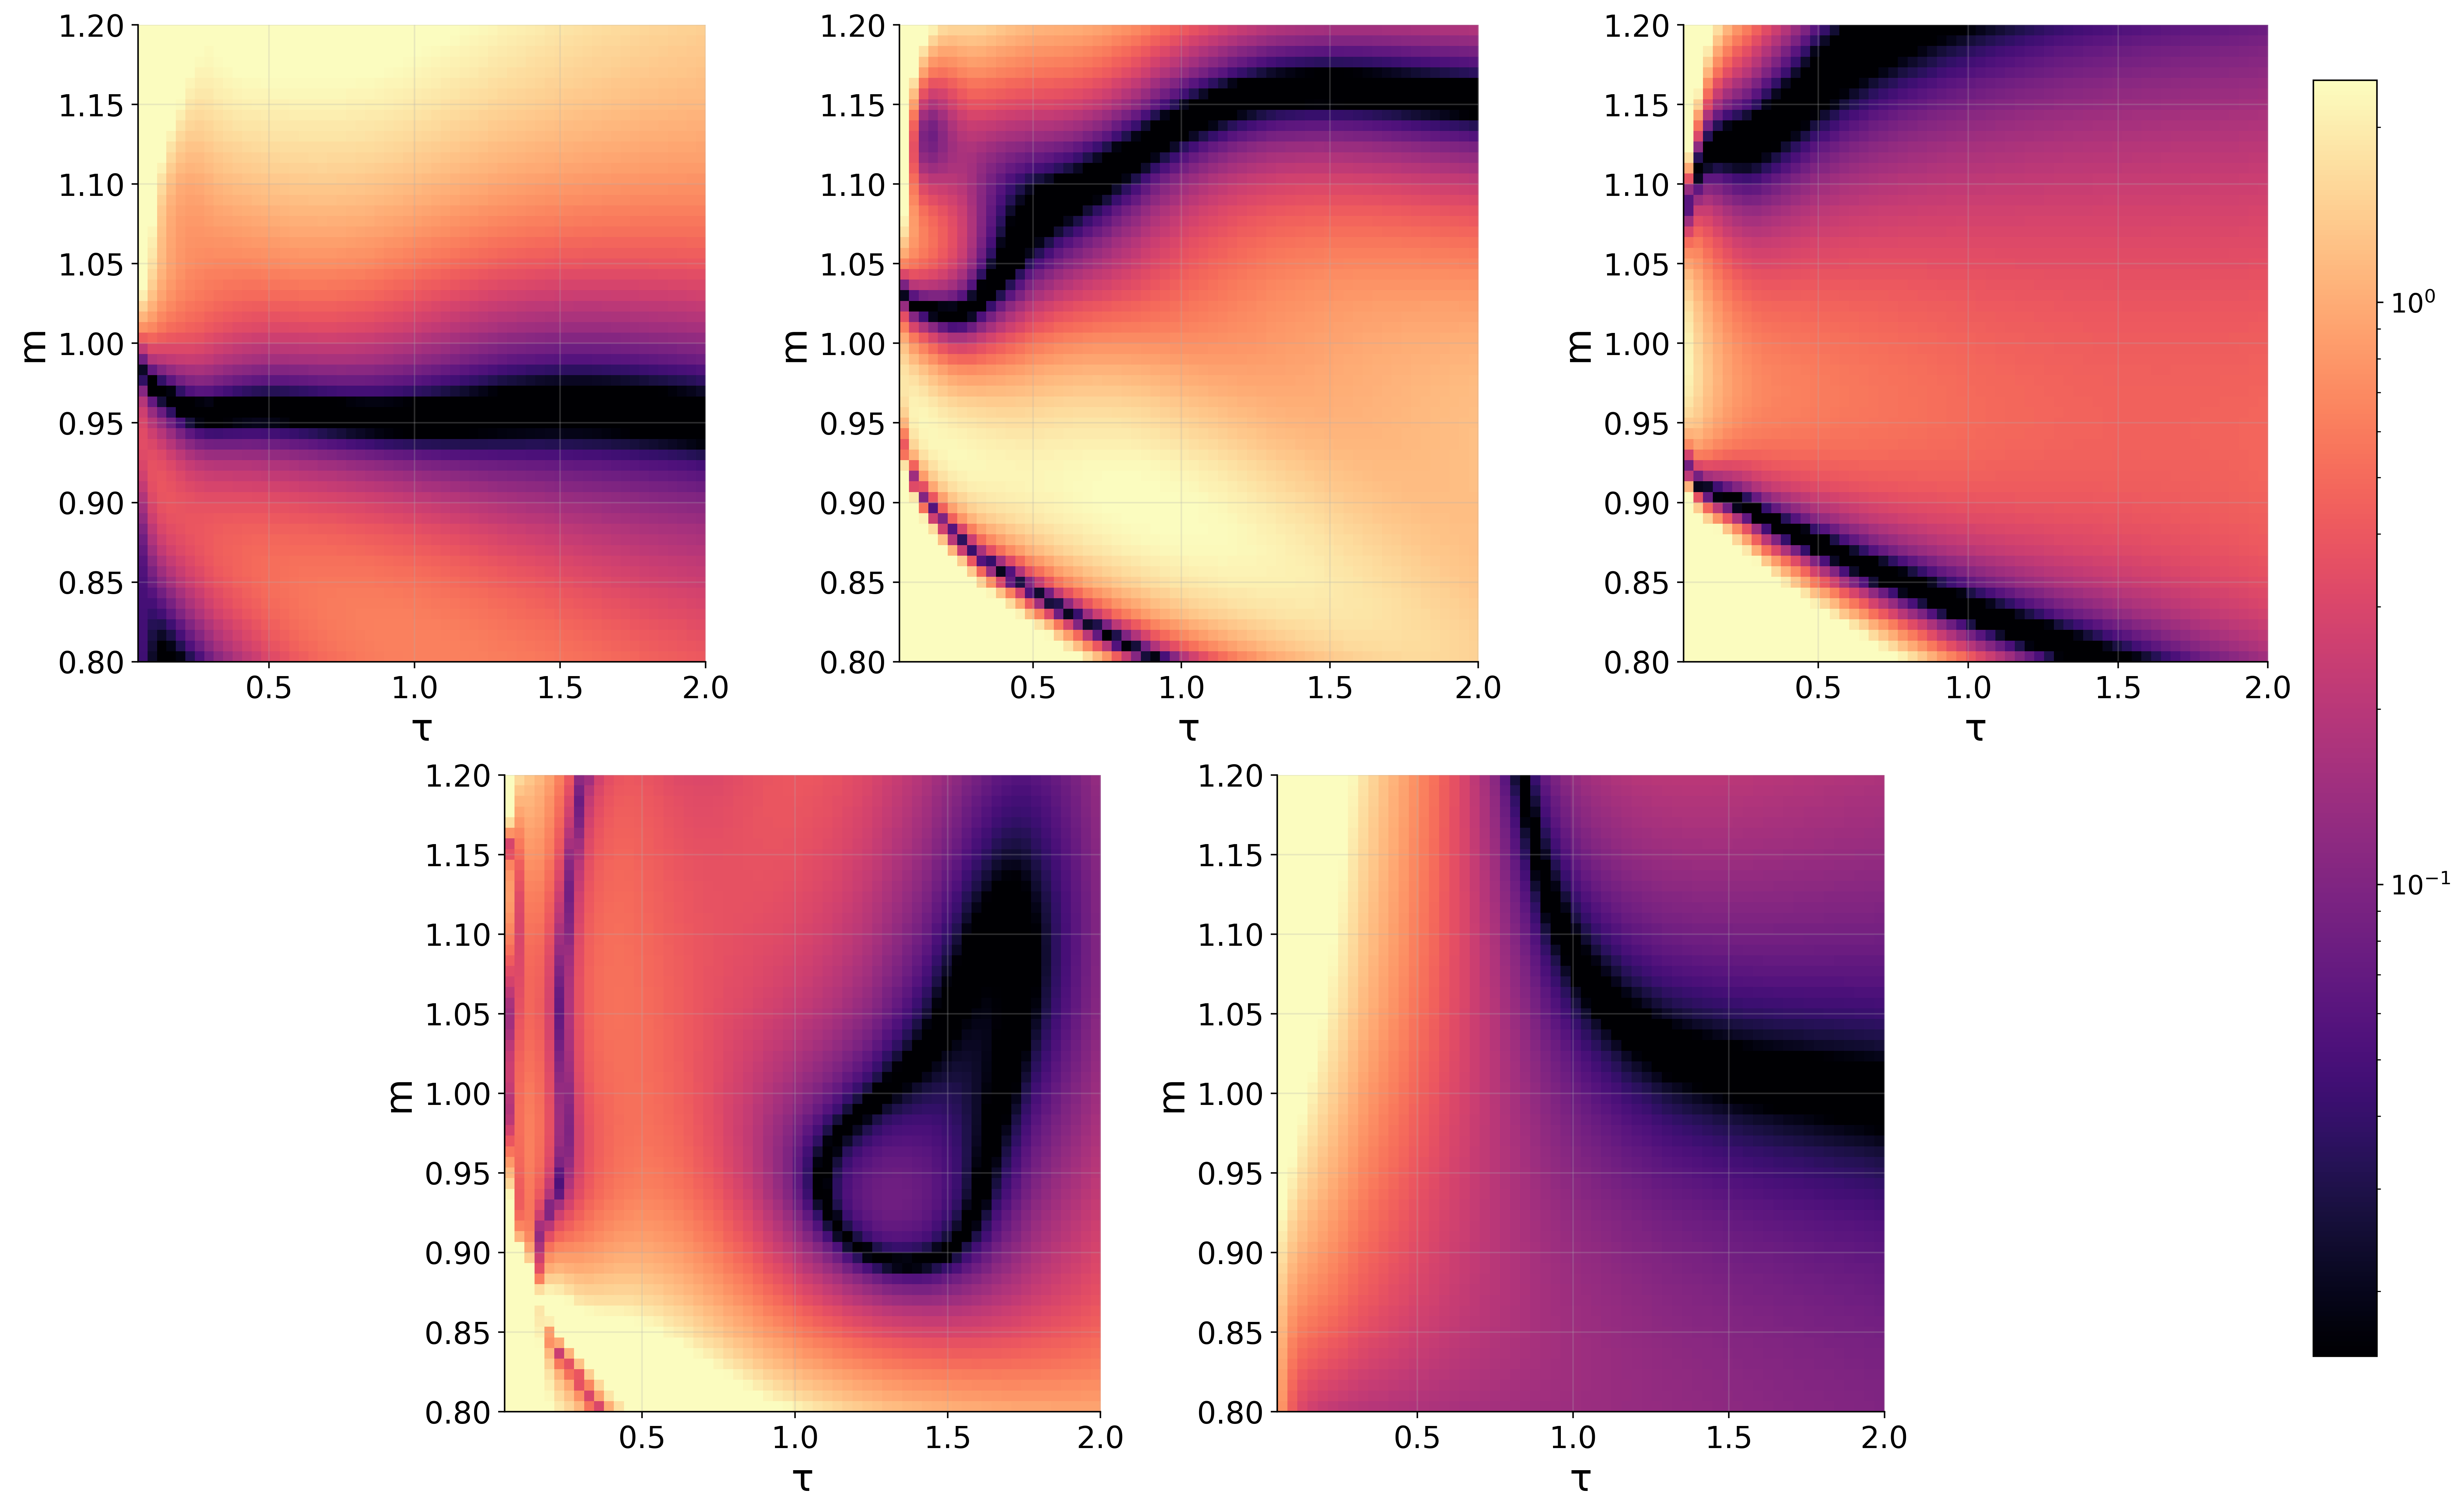
\includegraphics[width=1\textwidth]{figures/pinn/greeks/no_sobolev_rel_abs_error_maps_5greeks.png}
    \caption{Baseline PINN Greek relative-error maps.}
    \label{fig:no_sobolev_greeks_error_maps}
\end{figure}

\todos{Corregir figura comparativa: caption debe decir baseline--Sobolev y el label no puede duplicar el de la figura anterior.}
\begin{figure}[H]
    \centering
    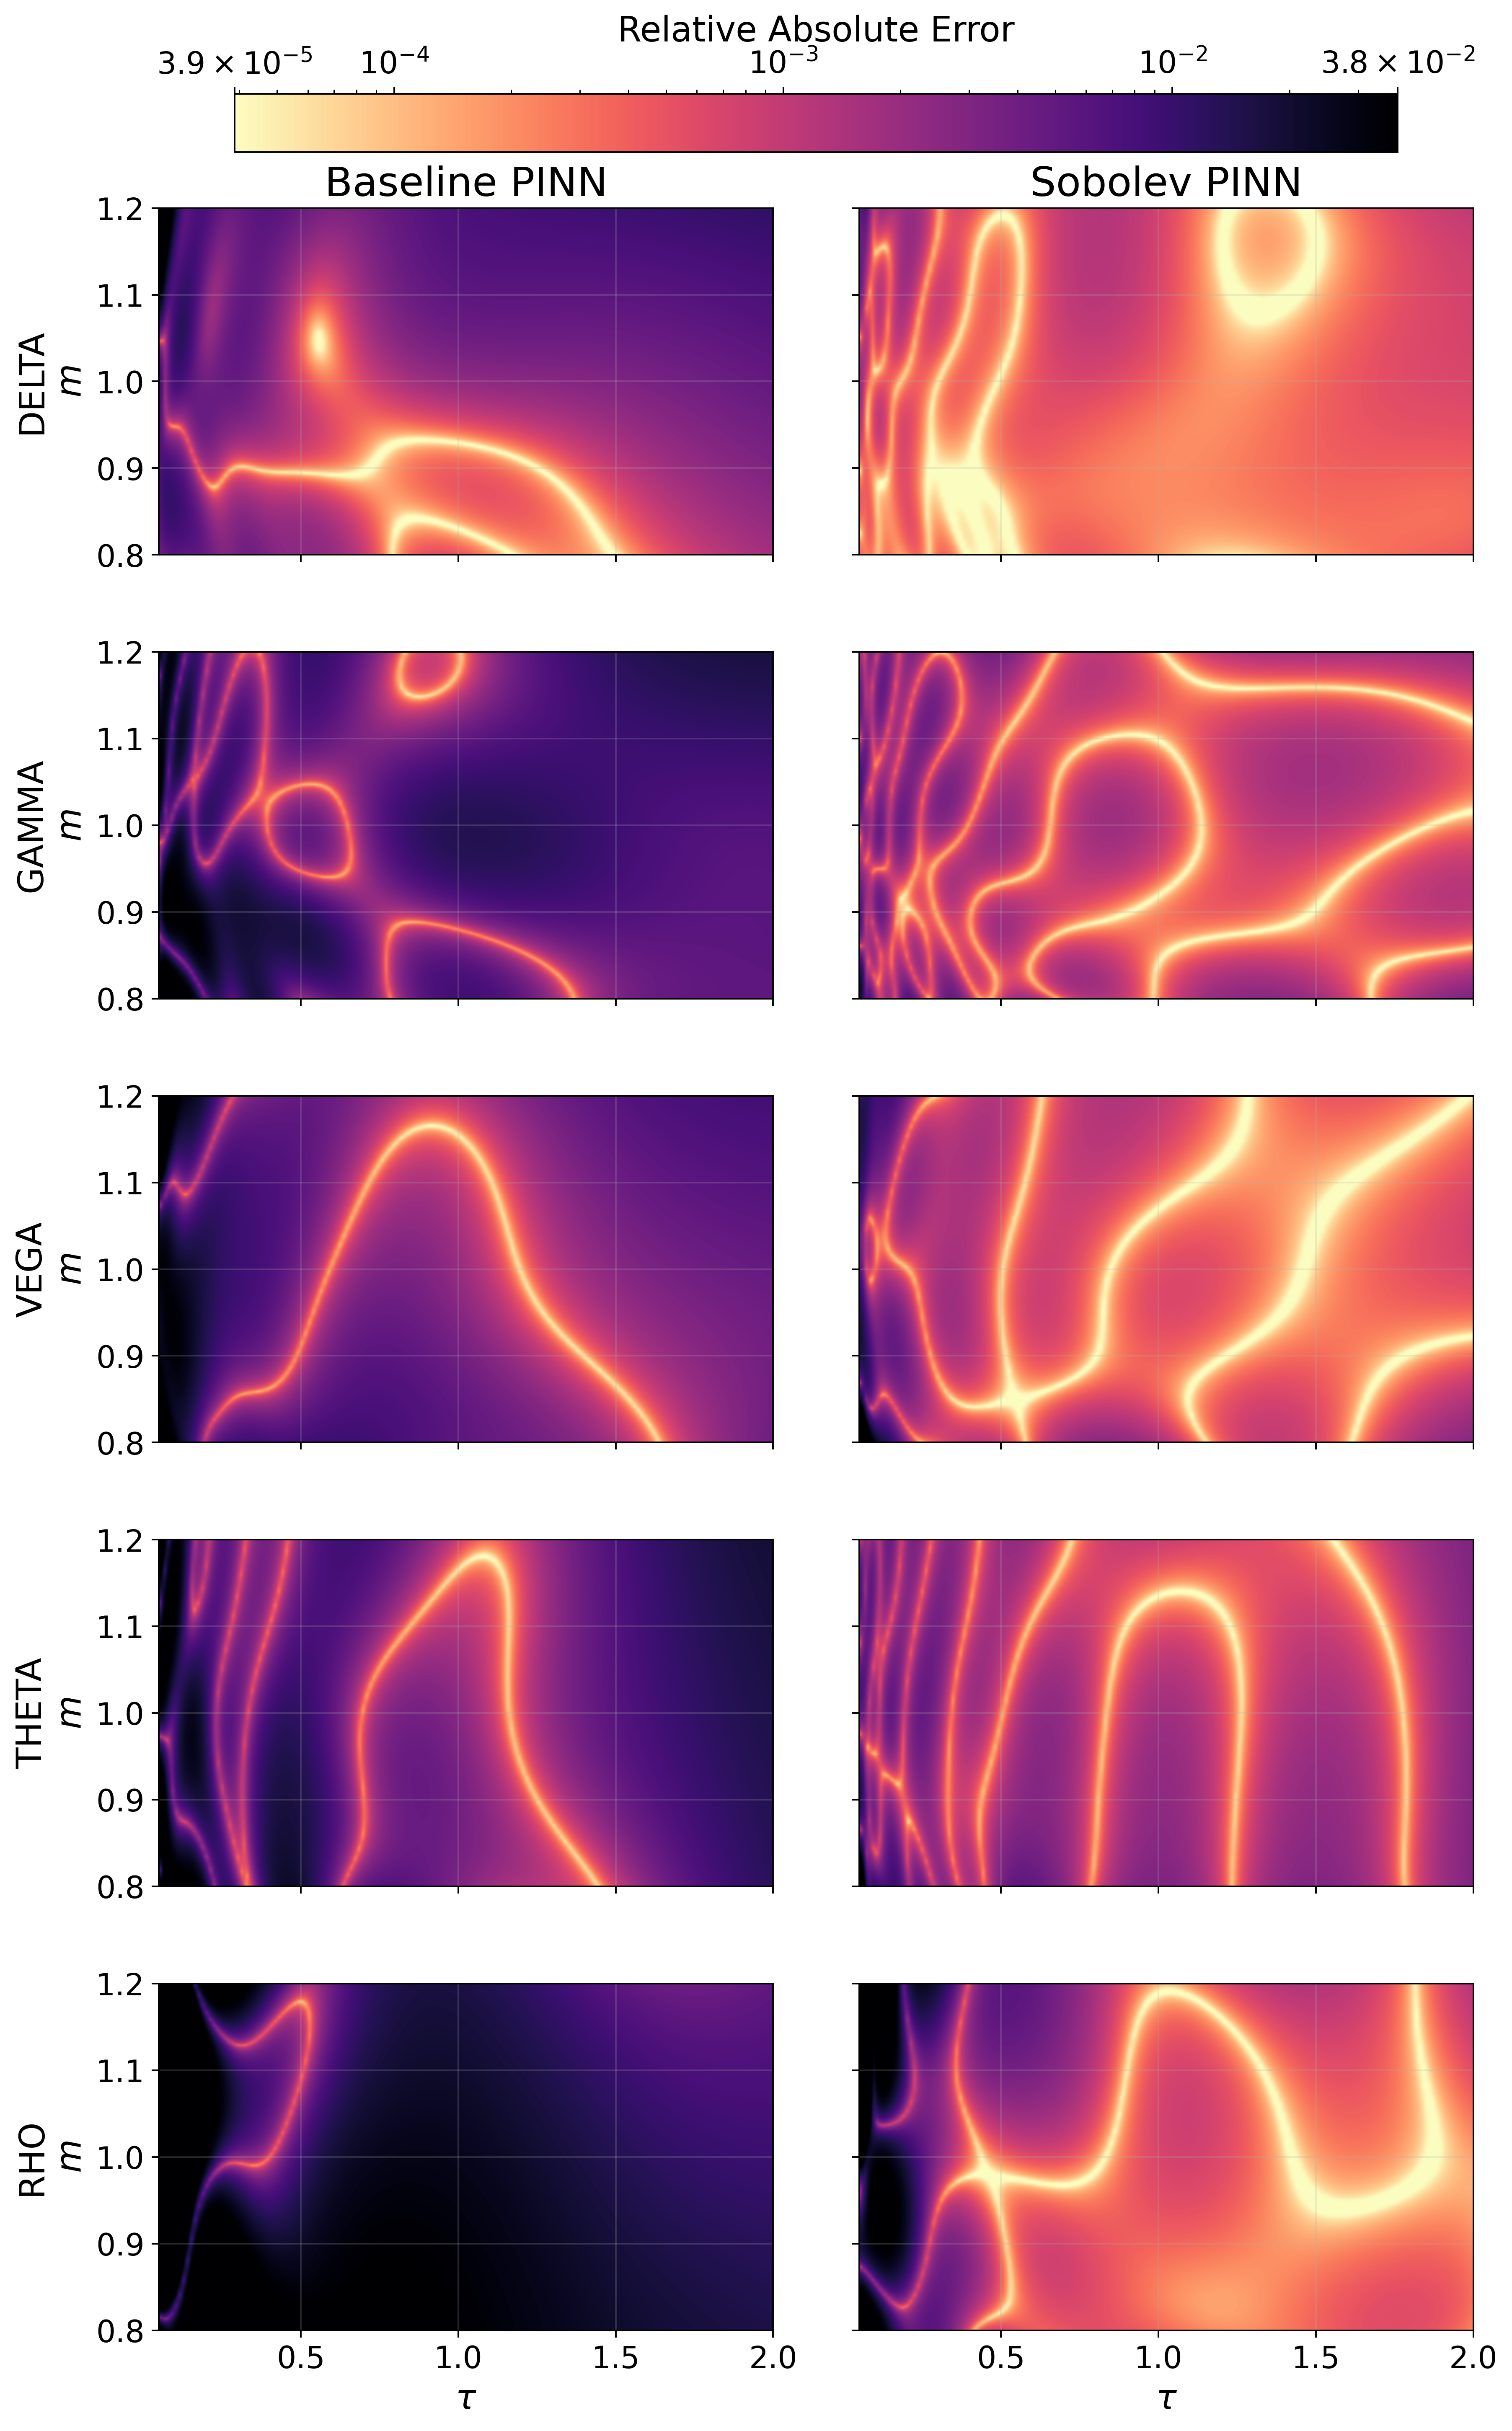
\includegraphics[width=0.90\textwidth]{figures/pinn/greeks/pinn_baseline_sobolev_greek_rel_error_maps_10panel.png}
    \caption{ADAPTAR}
    \label{fig:pinn_baseline_sobolev_greek_rel_error_maps}
\end{figure}

The baseline histogram panel complements this map-level view with error distributions. The heaviest tails appear in GAMMA and VEGA, while DELTA, THETA, and RHO are comparatively tighter. This confirms that the baseline model captures coarse sensitivity structure but still exhibits non-negligible extreme deviations in the hardest derivatives.

\begin{figure}[H]
    \centering
    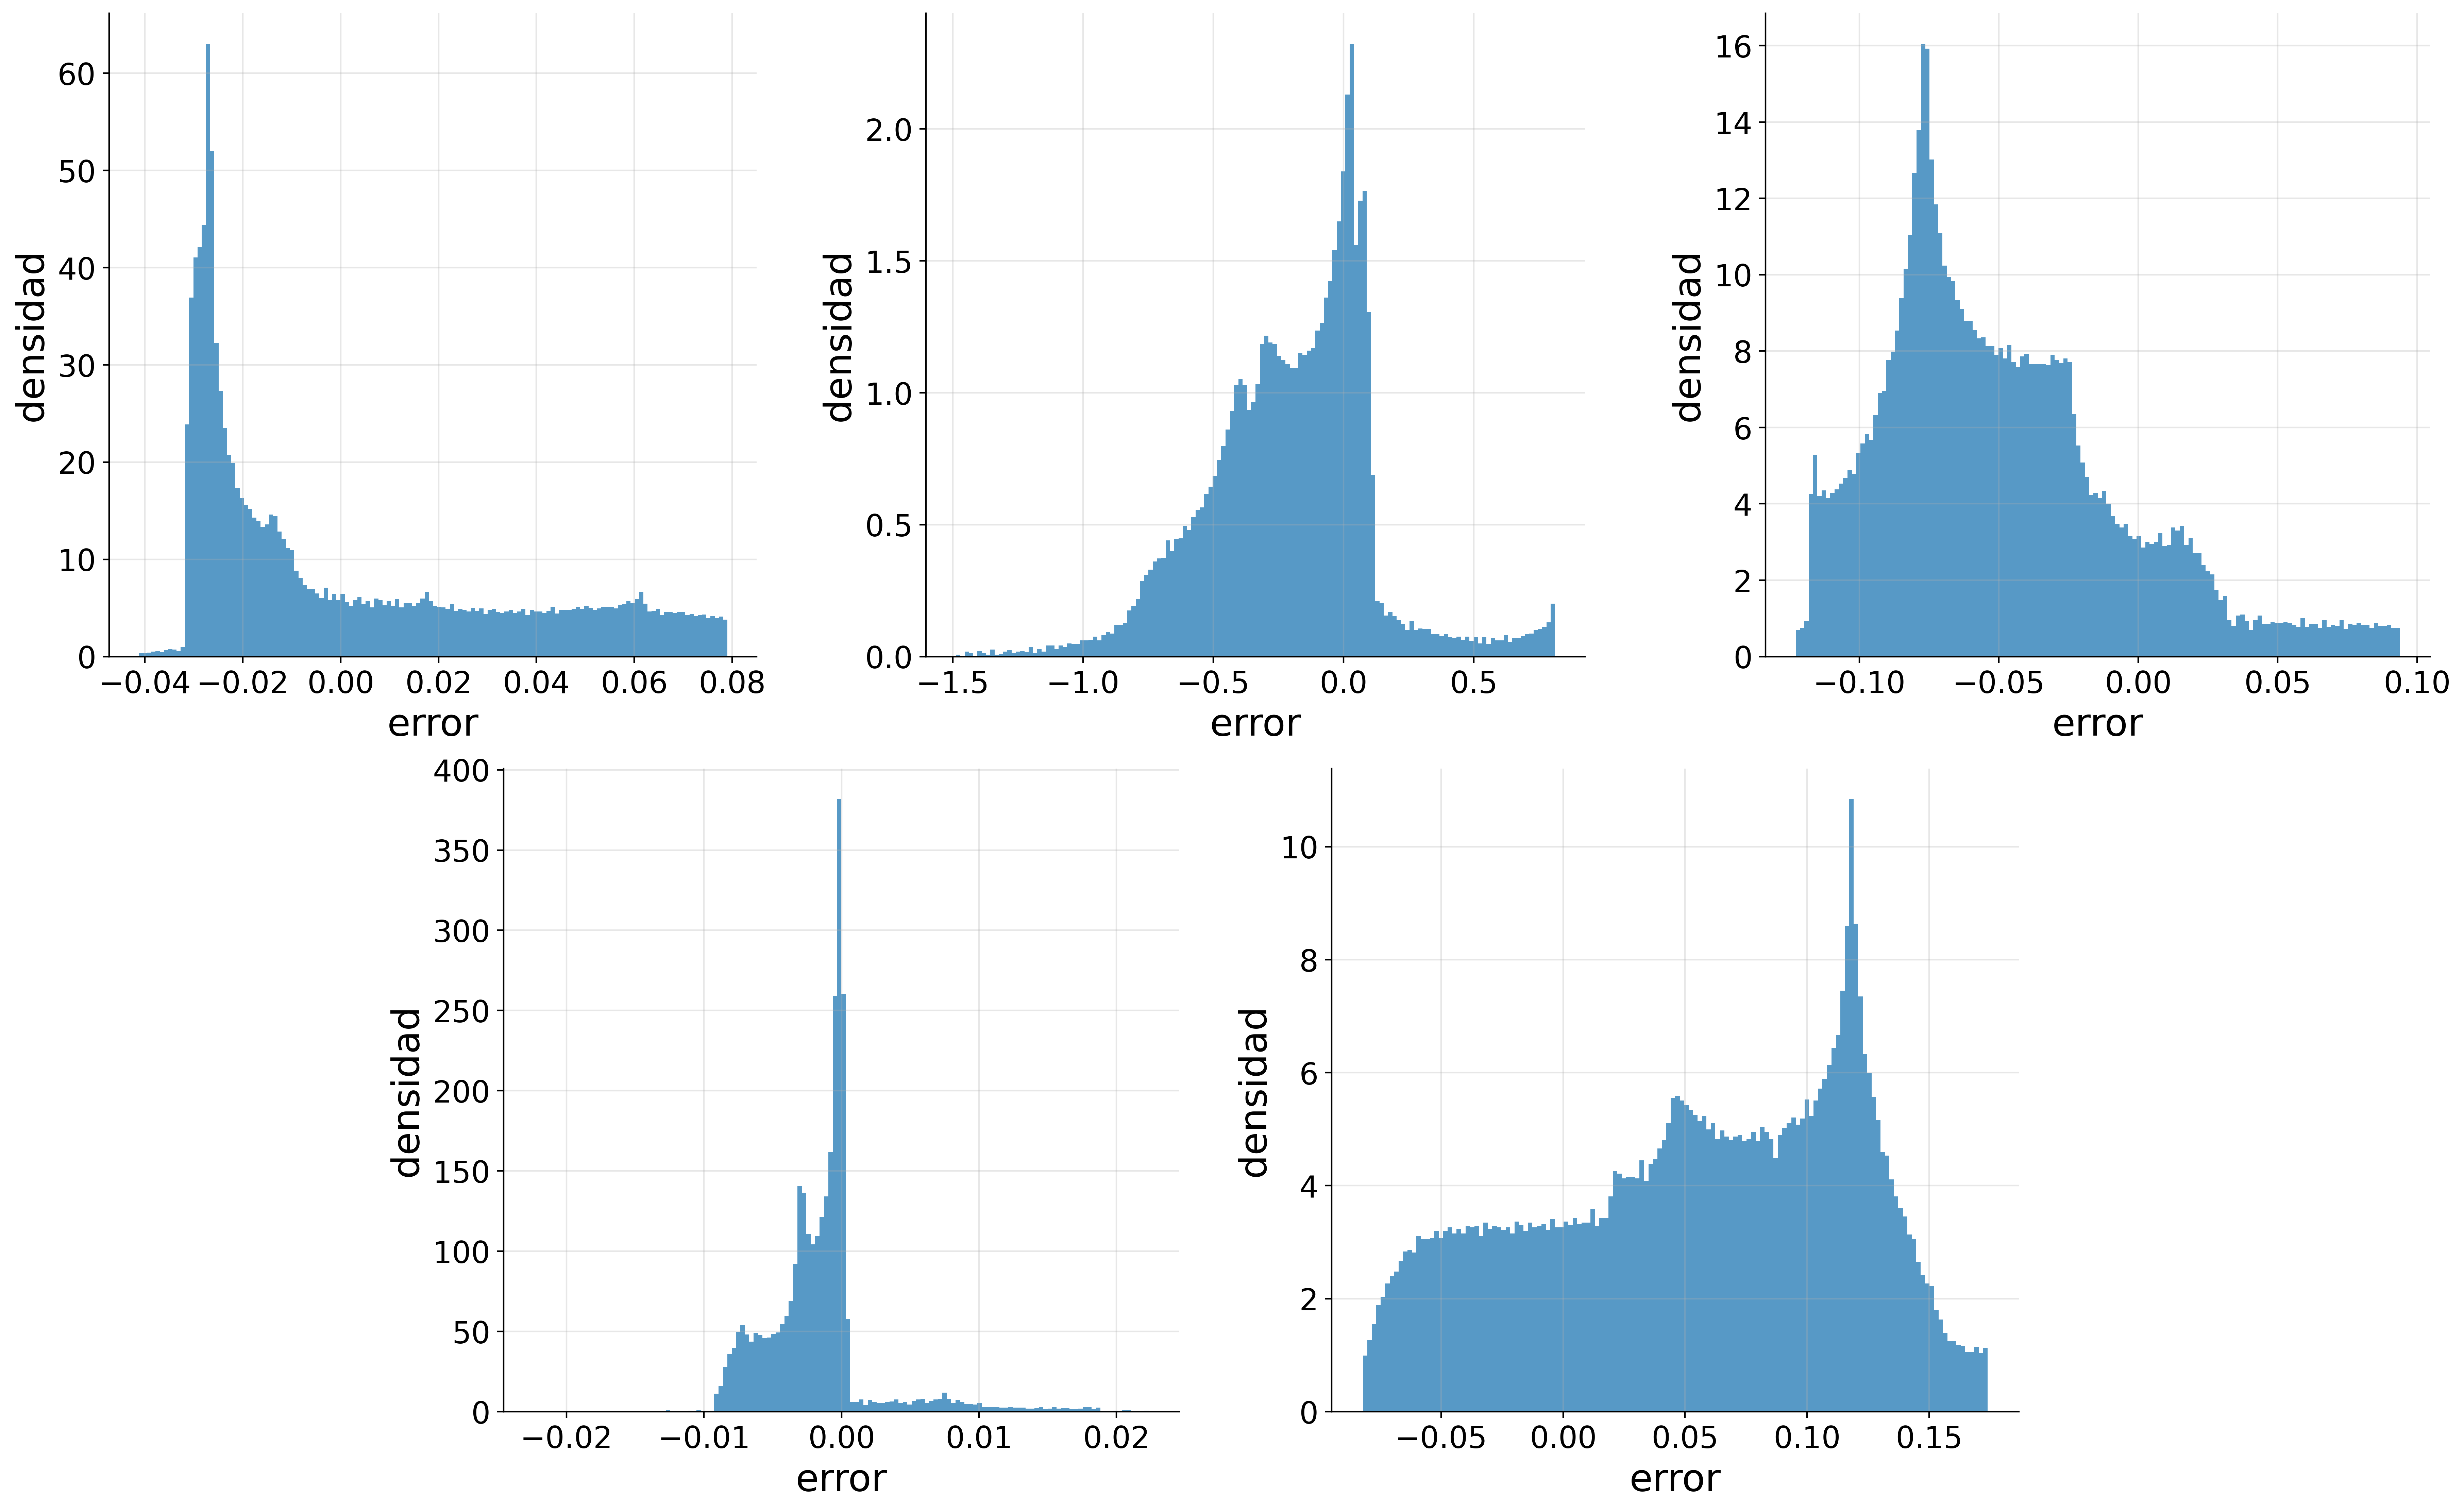
\includegraphics[width=1\textwidth]{figures/pinn/greeks/no_sobolev_error_hist_5greeks.png}
    \caption{Baseline PINN Greek error histograms.}
\end{figure}


After adding Sobolev terms, Figure~\ref{fig:sobolev_greeks_error_maps} shows a clear contraction of high-error regions across all Greeks. The strongest visual improvement appears in GAMMA and VEGA, where problematic zones become much smaller and less intense than in the baseline maps. This spatial change is consistent with the order-of-magnitude RMSE reductions reported in Table~\ref{tab:ablation_metrics_by_greek}.

\begin{figure}[H]
    \centering
    
\includegraphics[width=1\textwidth]{figures/pinn/greeks/sobolev_rel_abs_error_maps_5greeks.png}
    \caption{Sobolev PINN Greek relative-error maps.}
    \label{fig:sobolev_greeks_error_maps}
\end{figure}


The same effect appears in Figure~\ref{fig:sobolev_error_histograms}: Sobolev training narrows the distributions and reduces tail mass, so large deviations become less frequent for all five Greeks compared with the baseline histogram panel. The tail compression is particularly visible in GAMMA and VEGA, where baseline outliers were most persistent.

\begin{figure}[H]
    \centering
    
\includegraphics[width=1\textwidth]{figures/pinn/greeks/sobolev_error_hist_5greeks.png}
    \caption{Sobolev PINN Greek error histograms.}
    \label{fig:sobolev_error_histograms}
\end{figure}

\todos{Reubicar o eliminar este histograma overlay; si se mantiene, quitar TODO de la caption y explicar su papel.}
\begin{figure}[H]
    \centering
    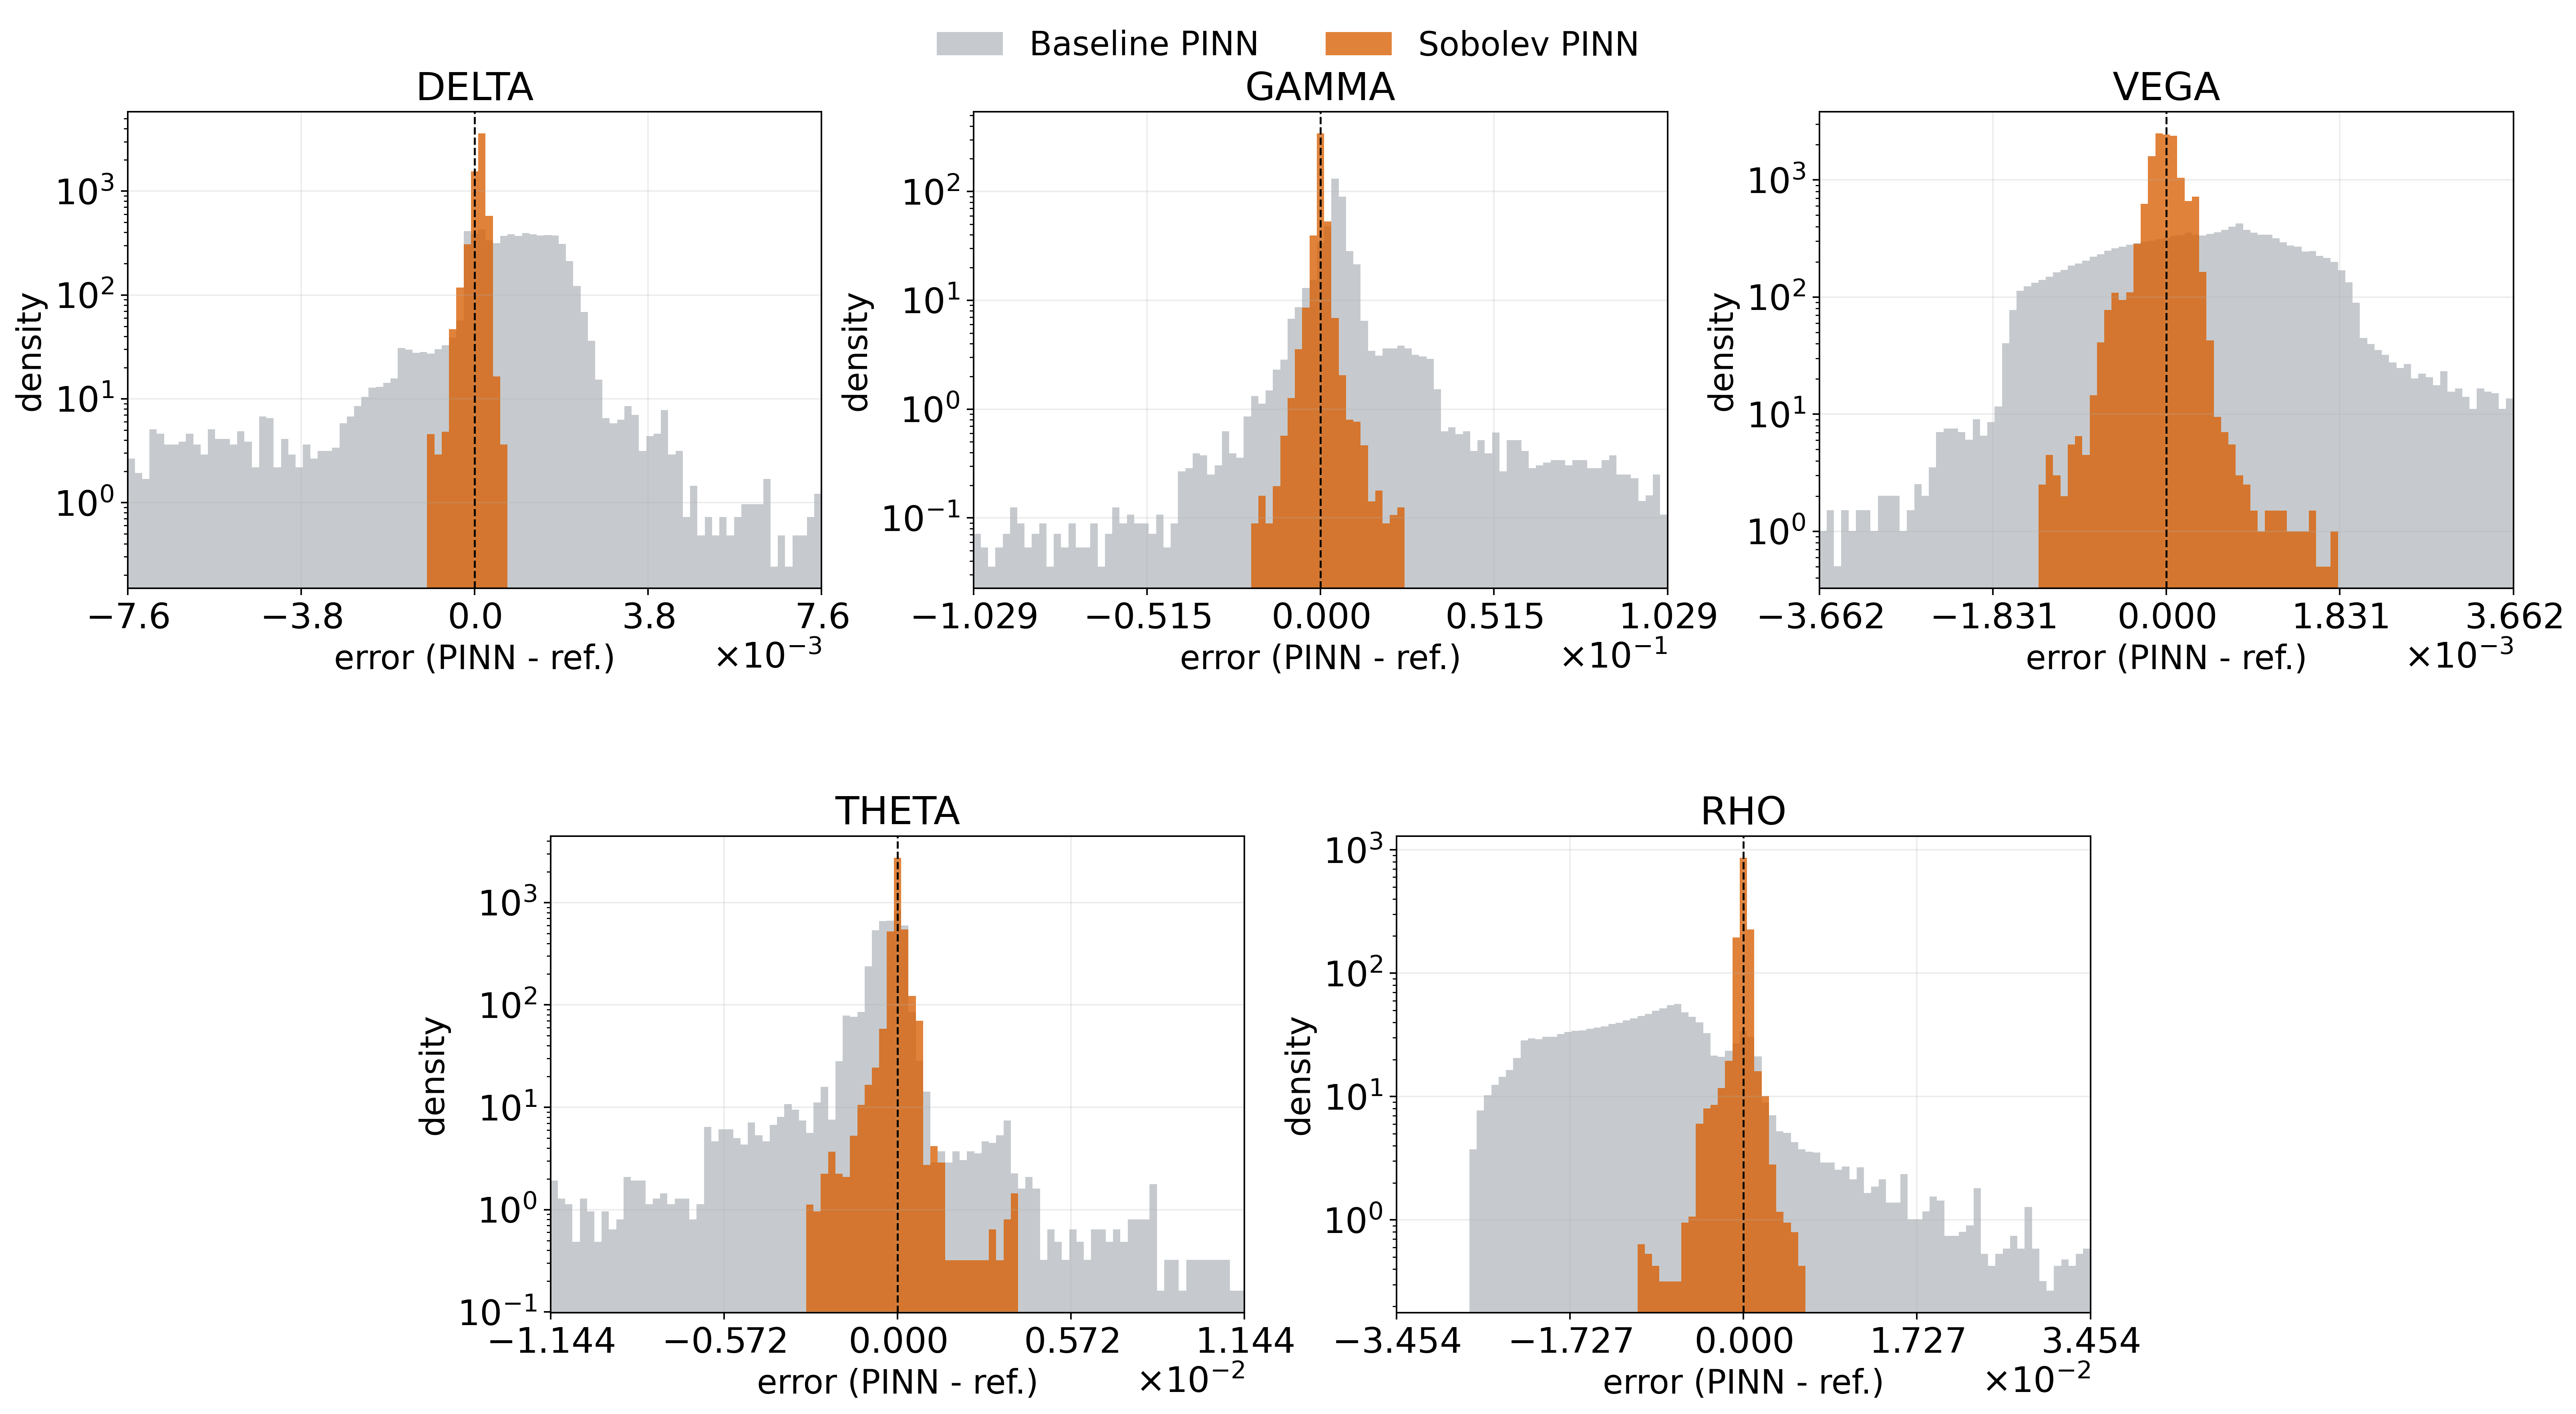
\includegraphics[width=1\textwidth]{figures/pinn/greeks/baseline_vs_sobolev_error_hist_overlay_logy_5greeks.png}
    \caption{\textbf{TODO: REUBICAR / AJUSTAR CAPTION.} Baseline--Sobolev Greek error histograms with overlaid log-density scale.}
    \label{fig:todo_baseline_sobolev_error_histograms}
\end{figure}


The two-phase optimization schedule used in this ablation trains epochs \(0\) to \(4000\) without Sobolev terms, then activates Sobolev augmentation from epoch \(4000\) onward. Together, the diagnostics indicate that Sobolev augmentation improves local derivative fidelity, not just aggregate scalar scores, while keeping the runtime overhead limited.

\subsection{Analytic Control Variate: Local Improvement In Difficult Regions}

\todos{Renombrar esta subseccion como PINN Sobolev+ACV si este es el quinto modelo final; explicar exactamente que componente ACV se anade al Sobolev.}
An additional Greek-focused diagnostic was run in parallel with the Sobolev study using an analytic-control-variate (ACV) hard patch. The accepted best-gate candidate keeps the frozen baseline PINN, adds a local Black--Scholes put control variate around the short-maturity ATM layer \cite{black_scholes_1973}, and initializes the residual network at zero without residual training. Consequently, the result isolates the effect of the structural control variate rather than an extra supervised Greek fit.

In this diagnostic, ``hard'' refers to the short-maturity ATM region
\[
\mathcal{D}_{\mathrm{hard}}
=\{(m,\tau):|\log(m)|<0.03,\ \tau<0.05\},
\]
which is precisely the neighborhood where the terminal put payoff kink at \(m=1,\tau=0\) creates the strongest curvature stress for Gamma estimation.

\begin{table}[H]
    \ttabbox[\FBwidth]
    {\caption{ACV control-variate diagnostic against the ablation baseline.}\label{tab:acv_control_variate_ablation}}
    {\begin{tabular}{|P{4.2cm}|P{3.0cm}|P{3.0cm}|}
        \hline
        \textbf{Metric} & \textbf{Baseline PINN} & \textbf{ACV control variate} \\
        \hline
        Price RMSE & \(4.269\times10^{-3}\) & \(4.235\times10^{-3}\) \\
        \hline
        Delta RMSE & \(3.381\times10^{-2}\) & \(3.269\times10^{-2}\) \\
        \hline
        Gamma RMSE & \(5.348\times10^{-1}\) & \(4.040\times10^{-1}\) \\
        \hline
        Hard Delta RMSE & \(8.729\times10^{-2}\) & \(1.288\times10^{-2}\) \\
        \hline
        Hard Gamma RMSE & \(4.992\) & \(6.446\times10^{-1}\) \\
        \hline
        Hard \(p_{99}\) Gamma error & \(17.643\) & \(1.612\) \\
        \hline
        \multicolumn{3}{l}{Source: Own elaboration based on ablation-study outputs.}
    \end{tabular}}
\end{table}

The control variate is therefore the strongest candidate in the ablation table for full Delta RMSE, full Gamma RMSE, hard-region Delta RMSE, hard-region Gamma RMSE, and hard \(p_{99}\) Gamma error. The result should still be read cautiously near the terminal payoff kink: the remaining Gamma error is concentrated in the short-maturity ATM layer, and the extremely short bucket \(\tau<5\times10^{-4}\) still requires separate validation of the semi-analytical Gamma reference before making stronger claims there.
\todos{Revisar consistencia: si el modelo final es PINN Sobolev+ACV, la tabla debe comparar baseline, Sobolev y Sobolev+ACV bajo el mismo protocolo.}

%%%%%%%%%%%%%%%%%%%%%%%%%%%%%%%%%%%%%%%%%%%%%%%%%
\section{Computational Cost And Model Roles}
\label{sec:cross_model_computational_comparison}
\todos{Reescribir comparacion final por familias y roles, no como pipeline lineal: ANN baseline/Sobolev frente a PINN baseline/Sobolev/Sobolev+ACV.}
This section summarizes the end-to-end pipeline in operational order, emphasizing where each model contributes and how computational cost is distributed.

First, market calibration is driven by the ANN pricer plus the CaNN optimization loop. The ANN stage provides fast implied-volatility evaluations (\(\approx 8.43\times10^5\) points/s), while CaNN concentrates cost in iterative inverse fitting. The retained Sobolev calibration reaches quote-level residual RMSE \(6.08\times10^{-6}\) and improves all reported Liu et al. parameter errors on the replicated \(35\)-quote benchmark, while the ANN baseline calibration remains the direct Liu-style reference.

Second, the calibrated market state \((\rho,\kappa,\gamma,\bar v,v_0)\) is injected into the parametric PINN pricing stage. On the final local fixed-grid pricing diagnostic, baseline PINN pricing reaches MSE \(9.43\times10^{-8}\), RMSE \(3.07\times10^{-4}\), and MAPE \(0.28\%\), while the Sobolev variant reaches MSE \(5.33\times10^{-8}\), RMSE \(2.31\times10^{-4}\), and MAPE \(0.18\%\). A separate broader repeated-evaluation benchmark is used only to quantify throughput: in that setting, the baseline PINN runs at approximately \(4.91\times10^5\) points/s, whereas COS runs at approximately \(87.36\) points/s, so the PINN remains several orders of magnitude faster in repeated evaluation mode.

Third, Greek extraction is performed on top of the same calibrated parameter state. The baseline PINN Greek pass runs at \(\approx 9.48\times10^3\) points/s, while the Sobolev variant runs at \(\approx 8.60\times10^3\) points/s (about \(9.3\%\) slower) and substantially improves derivative accuracy (for example, GAMMA RMSE from \(3.85\times10^{-1}\) to \(8.94\times10^{-3}\), VEGA RMSE from \(6.55\times10^{-2}\) to \(3.17\times10^{-3}\)). In the separate hard-region ablation, the ACV control variate gives the best Delta/Gamma metrics, reducing hard Gamma RMSE from \(4.992\) to \(6.446\times10^{-1}\) and hard \(p_{99}\) Gamma error from \(17.643\) to \(1.612\).

Pipeline-level error should be read as stagewise bounds, not as a single scalar. The ANN and CaNN stages control IV-space mismatch used for calibration, pricing quality is validated in price space against COS, and Greek quality is validated in derivative space. Since these are different output spaces and objectives, the most reliable reading is the per-stage error envelope reported above and in Sections~\ref{sec:ann_pricer_performance}--\ref{sec:pinn_greeks_performance}.
\todos{Cerrar con una lectura tipo: ANN Sobolev es el resultado fuerte para griegas supervisadas; PINN Sobolev+ACV es mejora localizada en el bloque physics-informed.}
